
\section{Über dieses Dokument}
\label{sec:orgcce6e7f}

\subsection{Beschreibung}
\label{sec:org2668df1}

Diese Arbeit hat zum Ziel, die Planung und Erstellung einer grafischen
Oberfläche zum einfachen Bedienen der Software \gls{borg} \footcite{borgbackup},
durchzuführen sowie zu dokumentieren.

\subsection{Zweck und Inhalt}
\label{sec:org74e290b}

Zweck dieses Dokumentes ist die vollständige und nachvollziehbare Dokumentation
zur Diplomarbeit von Andreas Zweili.

\subsection{Aufbau}
\label{sec:org3536775}

Inhalte sind in der Regel chronologisch sortiert, vom ältesten zum jüngsten
Ereignis, und nach Kapiteln getrennt. An gewissen Stellen kann die
chronologische Reihenfolge allenfalls nicht gewährleistet werden.

\subsection{Lizenz}
\label{sec:org3bc24f6}

Dieses Dokument wurde von Andreas Zweili im Rahmen der Diplomarbeit an der IBZ
Schule erstellt und steht unter der \gls{cc} BY-SA 4.0 \footcite{cc} Lizenz.
Dadurch darf die Arbeit unter Beibehalten der Lizenz kopiert und
weiterverarbeitet werden. Zusätzlich muss der Urheber genannt werden.

\section{Initialisierung}
\label{sec:orgdbad29f}
\subsection{Vision}
\label{sec:orgb4650e5}

Die Software soll \gls{borg} für den durchschnittlichen Computer User zugänglich
machen. Backups sollen dabei schnell und unkompliziert erstellt werden können.
Auch die Möglichkeit automatischer im Hintergrund laufender Backups soll dem
User gegeben sein, damit die Hürde für Backups so tief wie möglich gehalten
wird.

Die besten Backups sind solche, bei denen man gar nicht mehr weiss, dass man sie
hat bis man sie braucht.

\subsection{Ausgangslage}
\label{sec:org65d9768}

\gls{borg} ist deshalb interessant, weil es während einem Backup relativ
wenig Ressource im Vergleich zu anderen Systemen benötigt und schon relativ
lange aktiv entwickelt wird. Dadurch ist es im Alltag geprüft worden.
Des Weiteren bietet \gls{borg} die Funktion für Verschlüsselung, was es einem User
ermöglicht die Daten auf einem unsicheren Cloud Speicher abzulegen.

Des Weiteren speichert \gls{borg} die Daten mit Block basierter \gls{dedup} ab. Dies
hat den riesigen Vorteil, dass bei einem Backup nur die Änderungen auf
Block-Ebene gespeichert werden und nicht jedes Mal die ganze Datei kopiert
werden muss.

Damit ermöglicht die Software auch Backups von sehr grossen Dateien, wie Videos
oder Disk Images von virtuellen Maschinen, in mehreren Versionen. Ohne dabei
jedoch signifikant mehr an Speicher zu benötigen. Zusätzlich werden die Backups
dadurch rasend schnell ausgeführt. Gerade dieses Feature macht \gls{borg} in den
Augen des Autors besonders interessant, da sich der durchschnittliche User
möglichst wenig mit Dingen wie Backups auseinandersetzen möchte. Umso besser
also, wenn sie schnell gehen und so wenig Speicherplatz wie möglich verbrauchen.

\gls{borg} wird jedoch komplett über die Kommandozeile bedient. Somit ist es für
normale Benutzer eher schwierig den Zugang zu der Software zu finden, geschweige
denn sie zu bedienen.

\gls{borg} bietet Entwicklern eine \gls{json}, \gls{api}, mit welcher sie, von \gls{borg}
ausgegebenen Dateien einfach weiterverarbeiten können.

\gls{borg} steht unter einer \gls{bsd} \footcite{bsd} Lizenz zur Verfügung und ist
somit gemäss den Richtlinien der Free Software Foundation
\gls{libre} \footcite{fsflicenses}.

Das Projekt muss dabei vom Studenten in Eigenarbeit und einer Zeit von 250
Stunden bis zum 18. März 2019 erarbeitet werden.

\subsection{Projektziele}
\label{sec:org3d20026}

\gls{borg} ist eine Kommandozeilen basierte Backup Software. Hauptziel dieser
Arbeit ist, ein \gls{gui} für die Software \gls{borg} zu entwickeln um die Nutzung
zu vereinfachen. Da \gls{borg} selber freie Software ist und mit freier Software
viel gute Erfahrungen gemacht wurden, soll das Projekt selber auch wieder
\gls{libre} sein. Zum einen, um der Community etwas zurückzugeben, des weiteren,
um anderen Entwicklern die Möglichkeit zu geben die Software zu verbessern und
weiter zu entwickeln.

Als Nebenziel soll mit dieser Arbeit auch die Verbreitung von freier
Software gefördert werden. Dies wird insbesondere dadurch erreicht, dass die
Software selbst unter der \gls{gpl} Version 3 \footcite{gplv3} veröffentlicht wird.
Wenn möglich soll während der Entwicklung auch hauptsächlich freie Software
verwendet werden, um aufzuzeigen das ein solches Projekte nicht zwingend von
proprietärer Software abhängig ist. Die gesamte Arbeit wird zudem zu jedem
Zeitpunkt öffentlich einsehbar sein. Der Quelltext der Dokumentation ist unter
diesem Link erreichbar: \url{https://git.2li.ch/Nebucatnetzer/thesis}

Die Entwicklung wird hauptsächlich auf einem Linux System stattfinden. Da
\gls{borg} einerseits hauptsächlich auf Unix Systeme ausgelegt ist und anderseits
die Hauptzielgruppe des Projektes auch auf Linux Usern liegt. Trotzdem sollen
im Projekt cross-plattform fähige Technologien eingesetzt werden, damit es in
der Zukunft möglich ist das Projekt auf andere Plattformen auszuweiten.

\subsubsection{Ziele inklusive Gewichtung}
\label{sec:org2ef9c2b}

Im Projektantrag wurden vorgängig die Ziele in der
Tabelle:(\ref{tab:org2ab4045}) definiert und entsprechend
gewichtet. Die Gewichtung wurde dabei so vorgenommen, dass Ziele mit einer
Muss-Gewichtung den Minimalanforderungen der zu entwickelnden Software
entsprechen. Die weiteren Ziele wurden von 5 bis 1 gewichtet. Die Bewertung 5
bedeutet, dass die Umsetzung sehr nützlich und oder wichtig für die Software
ist und daher in naher Zukunft zu implementieren ist. Ein Ziel mit einer tiefen
Bewertung sollte, wenn möglich, auch einmal in die Software integriert werden
und ist nicht unwichtig.

\begin{longtable}{|p{1cm}|p{9cm}|p{1.5cm}|p{2cm}|}
\hline
\textbf{Ziel-Nr.}\cellcolor[HTML]{C0C0C0} & \textbf{Zielsetzung}\cellcolor[HTML]{C0C0C0} & \textbf{Muss}\cellcolor[HTML]{C0C0C0} & \textbf{Wunsch}\newline (1-5, 5=sehr wichtig)\cellcolor[HTML]{C0C0C0}\\
\hline
\endfirsthead
\multicolumn{4}{l}{Fortsetzung von vorheriger Seite} \\
\hline

\textbf{Ziel-Nr.}\cellcolor[HTML]{C0C0C0} & \textbf{Zielsetzung}\cellcolor[HTML]{C0C0C0} & \textbf{Muss}\cellcolor[HTML]{C0C0C0} & \textbf{Wunsch}\newline (1-5, 5=sehr wichtig)\cellcolor[HTML]{C0C0C0} \\

\hline
\endhead
\hline\multicolumn{4}{r}{Fortsetzung nächste Seite} \\
\endfoot
\endlastfoot
\hline
1. & Die Anwendung setzt auf cross-plattform (Linux, Windows, OS X) fähige Technologien. & x & \\
\hline
2. & Die Anwendung steht unter der \gls{gpl} v3 der Öffentlichkeit zur Verfügung. & x & \\
\hline
3. & Der User kann mit weniger als 3 Klicks ein Backup ausführen. & x & \\
\hline
4. & Der User kann ein Archiv mit 3 Klicks löschen. & x & \\
\hline
5. & Der User kann unter Linux ein Archiv mit zwei Klicks "`read-only"' als Laufwerk mounten. & x & \\
\hline
6. & Der User kann ein Archiv wieder herstellen. & x & \\
\hline
7. & Der User kann den zu sichernden Pfad manuell in der Anwendung definieren. & x & \\
\hline
8. & Die Applikation holt ihre Konfiguration aus einer Plain-Text Datei. & x & \\
\hline
9. & Der User kann sein Repository auf einer Harddisk ablegen. & x & \\
\hline
10. & Die Anwendung exkludiert für einen Linux Computer sinnvolle Pfade bereits zu Beginn. & x & \\
\hline
11. & Die Archivliste wird nach einer Aktion automatisch aktualisiert. & x & \\
\hline
12. & Der User kann sein Repository auf einem über \gls{ssh} erreichbaren Server ablegen. &  & 5\\
\hline
13. & Der User kann den Namen eines Archivs selbst bestimmen. &  & 5\\
\hline
14. & Die Anwendung meldet transparent, wenn das Repository nicht erreichbar ist. &  & 5\\
\hline
15. & Die Anwendung meldet dem User, wenn noch ein \gls{hypervisor} am Laufen ist. &  & 5\\
\hline
16. & Die Anwendung leitet Meldungen von \gls{borg} transparent weiter. &  & 5\\
\hline
17. & Die Anwendung zeigt transparent an das \gls{borg} im Hintergrund bereits läuft. &  & 5\\
\hline
18. & Das Repository wird nach jedem Backup bereinigt. &  & 4\\
\hline
19. & Der User kann automatische Hintergrundbackups in der Anwendung konfigurieren. &  & 4\\
\hline
20. & Die Anwendung gibt dem User die Möglichkeit ein passendes Repository zu erstellen, wenn keines gefunden wird, die Anwendung jedoch bereits konfiguriert ist. &  & 4\\
\hline
21. & Die Applikation verwendet, wann immer möglich allgemeingültige Umgebungsvariablen. &  & 4\\
\hline
22. & Die Anwendung cached/speichert (evtl. zusätzliche) Informationen in einer Datenbank. &  & 3\\
\hline
23. & Die Anwendung zeigt beim ersten Starten einen Setup Wizard. &  & 3\\
\hline
24. & Der User kann sich mit 3 Klicks das Log eines Archivs anschauen. Nur möglich mit einer zusätzlichen DB. &  & 3\\
\hline
25. & Die Anwendung kann Systembenachrichtigungen auslösen. &  & 3\\
\hline
26. & Der User kann die Anwendung grafisch konfigurieren. &  & 3\\
\hline
27. & Der User kann entscheiden, ob ein gemountetes Archiv nach dem Schliessen der Applikation noch weiter verfügbar ist. &  & 2\\
\hline
28. & Der User kann das Repository wechseln. &  & 2\\
\hline
29. & Der User kann ein Archiv nach einer Datei oder einem Ordner durchsuchen. &  & 2\\
\hline
30. & Der User kann die "`Retention Policy"' konfigurieren. &  & 2\\
\hline
31. & Die Anwendung kann mit allen Features von \gls{borg} umgehen. &  & 2\\
\hline
32. & Die Applikation prüft, ob sie sich im richtigen Netzwerk befindet bevor sie eine Verbindung zum Server aufbaut. &  & 2\\
\hline
\caption{\label{tab:org2ab4045}
Projektziele}
\\
\end{longtable}
\newpage

\subsection{Projektabgrenzung}
\label{sec:org82d5209}

Die Anwendung beschränkt sich darauf Funktionen von \gls{borg} grafisch
darzustellen oder nützlich zu erweitern, soweit dies über die \gls{api} möglich
ist. Wie in Abbildung:(\ref{fig:org5ba804d}) zu sehen ist, werden die Aktionen effektiv
immer vom Borg Binary ausgeführt und nicht von der grafischen Oberfläche. Eine
Erweiterung von \gls{borg} ist nicht vorgesehen. Dies aus dem Grund das Backups,
Deduplikation und Verschlüsselung sowie deren korrekte Implementation komplexe
Themen sind und unbedingt nur von Experten angegangen werden sollten. Die
Auswirkungen von Fehlern sind sind schlicht zu gross.

Des Weiteren wird die Grundlage für eine kollaborative Entwicklung geschaffen.
Während der Laufzeit der Diplomarbeit werden jedoch keine Inputs aus der Borg
Community im Bezug auf die Entwicklung entgegengenommen.

Bugs von \gls{borg} welche während der Dauer der Diplomarbeit vom Studenten
entdeckt werden, wird dieser dem Projekt melden, jedoch nicht selber beheben.

\begin{figure}[htbp]
\centering
\includegraphics[width=.9\linewidth]{pictures/kontextdiagramm.pdf}
\caption{\label{fig:org5ba804d}
Kontextdiagramm des Borg GUI}
\end{figure}

\subsection{Projektmethode}
\label{sec:org7ae08c5}

Für das Projekt wurde die \gls{wasserfall} gewählt. Da nur eine
einzige Person am Projekt arbeitet, kann nur ein Task nach dem anderen
abgearbeitet werden und viele Aufgaben stehen in Abhängigkeit zueinander.
Somit macht das iterative Vorgehen der \gls{wasserfall} für dieses Projekt am
meisten Sinn.

\subsection{Konfigurationsmanagement}
\label{sec:org54092b2}

\subsubsection{Versionskontrolle}
\label{sec:org7cdfd56}

Die komplette Dokumentation, der Quellcode der Applikation sowie jegliche
zusätzlichen Dokumente, wie etwa die Zeitplanung, werden mittels der Software
\gls{git} versioniert. Thematisch zusammengehörende Änderungen werden in einem
\gls{commit} zusammengefasst. Somit ist jederzeit nachvollziehbar, was wann
geändert hat. Ein \gls{commit} sollte dabei gemäss dem Artikel von Chris Beams
"`How to write a Git \gls{commit} Message"' \footcite{commit} und in englischer
Sprache geschrieben sein.

Versionsnummern sind für die Applikation zum jetzigen Zeitpunkt noch nicht
vorgesehen. Sollten sie zukünftig einmal verwendet werden, soll eine
semantische Versionierung \footcite{semver} verwendet werden. Dabei ist eine
Versionsnummer immer nach diesem Schema aufgebaut, MAJOR.MINOR.PATCH. Bei
Änderungen wird die:
\begin{enumerate}
\item MAJOR Version erhöht, wenn man inkompatible Änderungen an der \gls{api} macht.
\item MINOR Version erhöht, wenn man Funktionalität hinzufügt, die
abwärtskompatibel ist.
\item PATCH Version erhöht, wenn man abwärtskompatibel Bug-Fixes hinzufügt.
\end{enumerate}
Eine Versionsnummer würde dann so aussehen Version 1.2.3.

Auf jeden Fall sollte, sofern möglich, immer nur lauffähiger Code im Master
Branch eingecheckt sein, damit der Master Branch immer eine funktionierende
Software repräsentiert. Dies gilt auch für das Repository der Dokumentation.
Der Master Branch der Dokumentation sollte maximal mit zwei Befehlen \texttt{make
clean} und \texttt{make} "`kompilierbar"' sein.

Als Software für die Versionskontrolle wurde \gls{git} \footcite{git} aus den
folgenden Gründen ausgewählt:

\begin{itemize}
\item Ist der de facto Standard bei Versionskontrollsoftware
\item Läuft auf allen gängigen Betriebssystemen
\item Es gibt gratis Services, die man nutzen kann (Github, Gitlab)
\item Ermöglicht es offline zu arbeiten und \glspl{commit} erstellen
\item Es steht bereits ein eigener \gls{git} Server zur Verfügung
\item \gls{git} ist aus vorhergehenden Projekten vertraut,
dadurch muss kein Aufwand betrieben werden, eine neue Software zu lernen.
Zusätzlich hat sich \gls{git} in den vorhergehenden Projekten als robuste
und schnelle Software erwiesen.
\item \gls{git} ist \gls{libre} unter der \gls{gpl} v2.
\end{itemize}

\subsubsection{Editor}
\label{sec:org99f5c71}

Sowohl bei der Dokumentation wie auch bei der Programmierung wurde
hauptsächlich der Editor GNU Emacs \footcite{emacs} verwendet. GNU Emacs ist mit
32 Jahren (seine Wurzeln reichen bis ins Jahre 1976 zurück) wohl eines der
ältesten noch aktiven Software Projekte. Emacs ist \gls{libre} unter der \gls{gpl}
v3. Emacs wurde gewählt, da es ein schneller, schlanker und sehr flexibler
Texteditor ist. Von normaler Textmanipulation über Taskmanagement bis zu Emails
schreiben ist alles möglich.

\subsubsection{Dokumentation}
\label{sec:org4b11da7}

Diese Dokumentation wurde in Org-mode \footcite{orgmode}, einer Erweiterung für
den Text Editor Emacs, geschrieben. Die Syntax von Org-mode erinnert an
Markdown. Org-mode bietet einem eine Vielzahl an Hilfen, inklusive dem
Erstellen von Tabellen und Spreadsheet Funktionen. Für die finale Version des
Dokuments kann Org-mode die ursprünglich Textdatei über \LaTeX{} in eine PDF Datei
exportieren.

\LaTeX{} \footcite{latex} ist eine Software, welche einem die Benutzung des
Textsatzsystems TeXs vereinfacht. \LaTeX{} wurde gegenüber einem "`What You See Is
What You Get"' (z.Bsp. MS. Word) Editor gewählt, weil es einem mit seiner Markup
Sprache erlaubt das Dokument in Textdateien zu erstellen, gerade für
Programmierer ist dies eine sehr interessante Lösung. Dadurch, dass \LaTeX{} auch
nur aus reinen Textdateien besteht, können die Dokumente auch ohne weiteres
in die Versionskontrollsoftware einchecken und die Entwicklung im Log
zurückverfolgen. \LaTeX{} ist \gls{libre} unter der \LaTeX{} Project Public
License.

Die Grafiken in diesem Dokument wurden hauptsächlich mit dem Vektor Grafik
Editor Inkscape \footcite{inkscape} erstellt. Inkscape ist \gls{libre} unter der
GNU Public License v3.

Die Diagramme wurden mit Draw.io \footcite{draw} erstellt. Draw.io ist \gls{libre}
unter Apache Lizenz Version 2.0 \footcite{apache} und kann sowohl als Desktop
Applikation wie auch als Webanwendung genutzt werden.

Beim Design der Arbeit wurden soweit als möglich die typographischen Regeln aus
dem Buch "`Practical Typography"' von Matthew Butterick \footcite{typo} angewandt.
Bei den Diagrammen wurden ausschliesslich Farben aus der von Google
entwickelten Design Sprache "`Material"' \footcite{material} eingesetzt.

\subsection{Zeitplanung}
\label{sec:org3e1f3c8}

Die detaillierte Zeitplanung ist dem Ganttchart in der Datei:\newline
\href{02\_Zeitplanung\_Andreas\_Zweili.html}{02\_Zeitplanung\_Andreas\_Zweili.html}
zu entnehmen. Bei der Zeitplanung wurde darauf geachtet, dass die Arbeit soweit
als möglich nicht mit dem Berufsleben kollidiert. An einem normalen Arbeitstag
wurde dabei damit gerechnet das ca. 2 Stunden Arbeit am Abend möglich sein
sollten. An einem arbeitsfreien Tag wurde mit 6 Stunden Arbeit gerechnet. Über
die Festtage wurden diverse Tage von der Planung ausgenommen, da es nicht
realistisch schien, dass an diesen Tagen die Arbeit signifikant vorwärts gehen
würde. Auch Schultage wurde nicht als Arbeitstage gerechnet.

Um die Arbeitslast zu verteilen, wurde vom 14. Januar bis zum 11. März auf der
Arbeitsstelle jeder Montag als frei eingegeben. Dadurch steht während des
Projektes etwas mehr Zeit zur Verfügung, als mit einer 100 Prozent
Arbeitsstelle möglich wäre.

\subsection{Controlling}
\label{sec:org208d93d}

Mit dem Controlling wird die Planung mit den effektiv verwendeten Ressourcen
verglichen und ausgewertet. Somit können für zukünftige Projekte Lehren gezogen
werden.

\subsubsection{Zeitaufwand}
\label{sec:org48b7af7}

Um den geschätzten Zeitaufwand mit dem effektiv geleisteten Aufwand zu
vergleichen wurde die Tabelle:(\ref{tab:orgdc653bf}) erstellt. Darin werden die beiden
Aufwände einander gegenübergestellt und grössere Abweichungen begründet.
Die Nummer vor jeder Aufgabe in der Tabelle korreliert dabei mit den
Aufgabennummern im Ganttchart.

\subsubsection{Ressourcen}
\label{sec:orgf32159d}

In der Tabelle:(\ref{tab:org0a7c4bd}) wurden die für die Arbeit benötigten Materialen
erfasst. Da es sich beim Projekt um ein reines Software Projekt handelt ist der
Material Aufwand entsprechend gering. Im Abschluss des Projektes werden die
geplanten Ressourcen den effektiv verwendeten gegenübergestellt.

\subsubsection{Kosten}
\label{sec:org7c0906b}

Werden die internen Lohnkosten des Projektleiters auf ca. 60 CHF pro Stunde
geschätzt (dies entspricht in etwa dem doppelten reelen Stundenlohn des
Projektleiters), ergeben sich gemäss der Berechnung in der
Tabelle:(\ref{tab:orgc5c17d7}), theoretische Kosten von 19080 CHF für die Umsetzung
dieser Arbeit. Die Kosten für die Entwicklung werden im Projekt jedoch nicht
berücksichtigt. Somit sind diese nur ein rein theoretischer Faktor.

\subsection{Projektrisiken}
\label{sec:orge68685e}

Das Risikomanagement dient dazu Risiken im Projekt zu erkennen und Massnahmen
zur Vermeidung zu definieren. Dadurch steht man Risiken nicht
unvorbereitet gegenüber, sollten sie eintreffen.

\subsubsection{Risikobeschreibung}
\label{sec:org5fac90a}

In der Tabelle:(\ref{tab:orgb156d31}) sind die Risiken des Projektes
gemeinsam mit ihren Gegenmassnahmen aufgelistet. Somit können gewisse Risiken
bereits vorher vermieden werden.

\begin{longtable}{|p{0.45\textwidth}|p{0.45\textwidth}|}
\hline
\textbf{Beschreibung}\cellcolor[HTML]{C0C0C0} & \textbf{Massnahmen}\cellcolor[HTML]{C0C0C0}\\
\hline
\endfirsthead
\multicolumn{2}{l}{Fortsetzung von vorheriger Seite} \\
\hline

\textbf{Beschreibung}\cellcolor[HTML]{C0C0C0} & \textbf{Massnahmen}\cellcolor[HTML]{C0C0C0} \\

\hline
\endhead
\hline\multicolumn{2}{r}{Fortsetzung nächste Seite} \\
\endfoot
\endlastfoot
\hline
Ein grösseres Problem in der Programmierung blockiert den Fortschritt. & Immer nur eine Sache auf einmal in der Code-Basis ändern, alle Fehler beheben und erst dann zur nächsten Aufgabe weitergehen.\\
\hline
Viel Arbeit an der Arbeitsstelle, dabei bleibt weniger Zeit für die Diplomarbeit. & Auf der Arbeit Freitage eingeben um die Last etwas zu verteilen. Projektplanung machen.\\
\hline
Know-How zur Umsetzung ist nicht vollständig vorhanden. & Gute Informationsbeschaffung im Internet, Büchern, etc.\\
\hline
Manuelle Tests brauchen zu viel Zeit. & Soviel wie möglich automatisieren. Dabei jedoch nicht den Fokus auf die eigentliche Entwicklung verlieren.\\
\hline
Die Programmierung des Programms benötigt zu viel Zeit. & Bei der Projektplanung genau definieren was die GUI Applikation beinhalten muss. Ziele definieren, Abgrenzungen treffen.\\
\hline
User haben keine Zeit für Benuterfreundlichkeitsstudie. & Vor gängig einen Termin abmachen.\\
\hline
\gls{borg} ändert fundamental seine \gls{api}. & Gegen eine fixe Version von \gls{borg} entwickeln.\\
\hline
\caption{\label{tab:orge8eb370}
Projektrisiken}
\\
\end{longtable}

\section{Analyse}
\label{sec:org61eed6c}
\subsection{SWOT-Analyse}
\label{sec:orgd8cfd66}

Die SWOT-Analyse ist eine Methode die Stärken, Schwächen, Chancen und
Gefahren zu erkennen, indem eine 4-Felder-Matrix ausgefüllt wird.

Grundlage einer guten SWOT Analyse ist eine klare Zieldefinition und
Fragestellung.. Die ausgefüllte SWOT-Analyse für dieses Projekt ist in der
Abbildung:(\ref{fig:org1eae858}) zu sehen.

\begin{figure}[htbp]
\centering
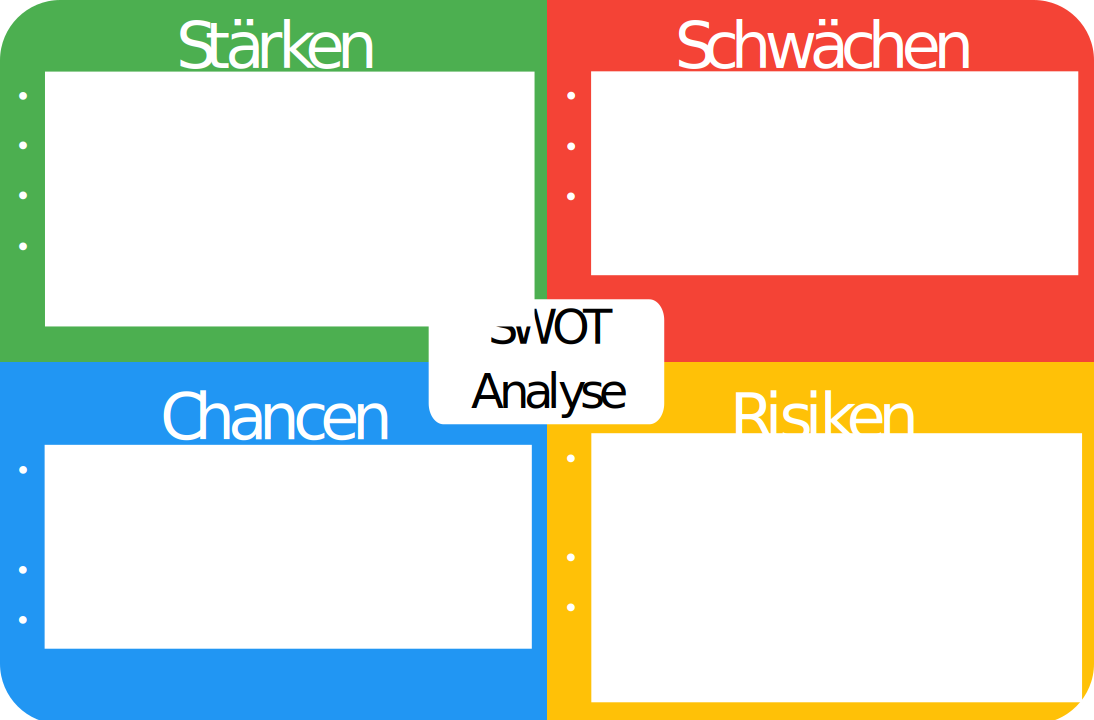
\includegraphics[width=.9\linewidth]{pictures/swot_analyse.pdf}
\caption{\label{fig:org1eae858}
SWOT Analyse des Projektes}
\end{figure}

\subsection{Umweltanalyse}
\label{sec:org9d9bddc}

Die Projektumwelt-Analyse ist eine Methode die Beziehungen,
Erwartungshaltungen und Einflüsse auf das Projekt durch interne und
externe soziale Umwelt zu betrachten und zu bewerten. Auf Grundlage
der Analyseergebnisse werden erforderliche Massnahmen zur Gestaltung
der Umweltbeziehungen abgeleitet. Die Gestaltung der
Projektumweltbeziehungen ist eine Projektmanagementaufgabe. In der
Tabelle:(\ref{tab:orgb66657b}) wurden die Anforderungen und Wünsche
mit Einschätzung der Wahrscheinlichkeit und der Einflussnahme aufgenommen.
Zusätzlich ist die Beziehung der Stakeholder zum Projekt noch in der
Abbildung:(\ref{fig:org96e2a60}) grafisch dargestellt.

Da das Projekt so ausgelegt ist, dass der Projektleiter es in Eigenarbeit
verwirklichen kann, ist der Einfluss der Stakeholder während der Umsetzung sehr
gering. Die User werden bei der Entwicklung mittels einer
Usability-Studie miteinbezogen und die \gls{borg} Community wird mit
regelmässigen Posts auf dem offiziellen Github Repository auf dem Laufenden
gehalten. Nach Ende der Diplomarbeit soll das Projekt für interessierte
Entwickler jedoch offen sein. Der Quellcode wird bereits während der Arbeit
öffentlich zur Verfügung gestellt.

\begin{figure}[htbp]
\centering
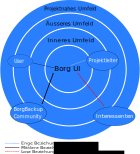
\includegraphics[width=.9\textwidth]{pictures/stakeholder_diagramm.pdf}
\caption{\label{fig:org96e2a60}
Stakeholder Diagramm}
\end{figure}

\newpage
\begin{landscape}
\begin{table}[htbp]
\centering
\begin{tabular}{|>{\columncolor[HTML]{EFEFEF}}p{0.8cm}|l|l|p{8cm}|l|}
\hline
\textbf{Nr}.\cellcolor[HTML]{C0C0C0} & \textbf{Stakeholder}\cellcolor[HTML]{C0C0C0} & \textbf{Einfluss}\cellcolor[HTML]{C0C0C0} & \textbf{Anforderung/Wünsche}\cellcolor[HTML]{C0C0C0} & \textbf{Wahrscheinlichkeit}\cellcolor[HTML]{C0C0C0}\\
\hline
1. & \gls{borg} Community & gering & Eine Applikation, die den Umfang von \gls{borg}\newline abdeckt & mittel\\
 &  &  & Open-Source & hoch\\
 &  &  & Mitspracherecht bei der Entwicklung & niedrig\\
\hline
2. & User & gering & Einfache Bedienbarkeit & hoch\\
 &  &  & Einmal einrichten und vergessen & mittel\\
\hline
3. & Interessenten & gering & Einfach verständliches Projekt Repository & hoch\\
 &  &  & Einfaches Setup zum Testen & hoch\\
\hline
4. & Projektleiter & hoch & Stabile Anwendung erstellen & mittel\\
 &  &  & Ein nachhaltiges Projekt starten & mittel\\
 &  &  & Anerkennung im fachlichen Umfeld & niedrig\\
\hline
\end{tabular}
\caption{\label{tab:orgb66657b}
Umweltanalyse}

\end{table}
\end{landscape}

\subsection{Risiko-Analyse}
\label{sec:org2347925}

Bei der Risiko-Analyse wird von einem durchschnittlichen Benutzer ausgegangen,
der zur Zeit noch keine Backups macht und beginnen möchte \gls{borg} zu nutzen, um
auf einer externen Harddisk seine Backups zu speichern.

In der Tabelle:(\ref{tab:orgb156d31}) sind die Risiken für das Szenario
aufgelistet und nummeriert. In der Abbildung:(\ref{fig:org2c84d03}) ist die
Bewertung des Ist-Risikos grafisch dargestellt und in der
Abbildung:(\ref{fig:org525577a}) ist das Soll-Risiko, welches mit dieser Arbeit
angestrebt wird, ebenfalls grafisch dargestellt.

Jedes Risiko wurde entsprechend der Tabelle:(\ref{tab:orgc24b878}) nach der
Wahrscheinlichkeit des Eintreffens bewertet und entsprechend der
Tabelle:(\ref{tab:org8a27a35}) nach seiner Auswirkung im Bezug auf die
Nützlichkeit der gemachten Backups.

Es sollte im Rahmen der Arbeit möglich sein die meisten Risiken zu verringern.
Da automatische Hintergrundbackups jedoch ein Kann-Ziel sind wir in dieser
Analyse nicht davon ausgegangen, dass man das Risiko Nr. 5 im Rahmen dieser
Arbeit reduzieren kann.
\begin{table}[H]
\centering
\begin{tabular}{|>{\columncolor[HTML]{EFEFEF}}p{0.1\textwidth}|p{0.8\textwidth}|}
\hline
\textbf{Nr.}\cellcolor[HTML]{C0C0C0} & \textbf{Beschreibung}\cellcolor[HTML]{C0C0C0}\\
\hline
1. & Der Benutzer hat noch nie die Kommandozeile verwendet und scheitert bereits an der Installation von \gls{borg}.\\
\hline
2. & Der Benutzer verwendet keine Verschlüsselung und verliert seine Harddisk.\\
\hline
3. & Der Benutzer speichert die Backups auf der internen statt der externen Harddisk.\\
\hline
4. & Der Benutzer löscht aus Versehen ein Backup.\\
\hline
5. & Der Anwender vergisst die Backups zu machen.\\
\hline
\end{tabular}
\caption{\label{tab:orgb156d31}
Risikobeschreibung}

\end{table}

\begin{figure}[H]
\centering
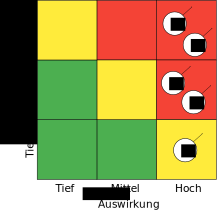
\includegraphics[width=9cm]{pictures/istrisiko.pdf}
\caption{\label{fig:org2c84d03}
Grafische Darstellung der Ist-Risikoanalyse}
\end{figure}

\begin{figure}[H]
\centering
\includegraphics[width=9cm]{pictures/sollrisiko.pdf}
\caption{\label{fig:org525577a}
Grafische Darstellung der Soll-Risikoanalyse}
\end{figure}


\begin{table}[H]
\centering
\begin{tabular}{l|l}
\textbf{Bewertung} & \textbf{Beschreibung: Wahrscheinlichkeit (W)}\\
\hline
1 = gering & Unwahrscheinlich, <20\%\\
2 = mittel & Mässig wahrscheinlich, 20-50\%\\
3 = hoch & Hohe Wahrscheinlichkeit > 50\%\\
\end{tabular}
\caption{\label{tab:orgc24b878}
Risikobewertung Wahrscheinlichkeit}

\end{table}

\begin{table}[H]
\centering
\begin{tabular}{l|l}
\textbf{Bewertung} & \textbf{Beschreibung: Auswirkung (A)}\\
\hline
1 = gering & Geringe Auswirkungen auf Nützlichkeit\\
2 = mittel & Mittlere Auswirkung auf die Nützlichkeit\\
3 = hoch & Hohe Auswirkung auf die Nützlichkeit\\
\end{tabular}
\caption{\label{tab:org8a27a35}
Risikobewertung Auswirkung}

\end{table}

\newpage
\subsection{Anforderungskatalog}
\label{sec:org90be6e5}

Der Anforderungskatalog entspricht 1:1 den Zielen, welche in der
Tabelle:(\ref{tab:org2ab4045}) definiert wurden. Im Zeitplan wurde der Fokus
hauptsächlich auf die Muss-Ziele gelegt. Ein paar der Kann-Ziele sind im
Konzept jedoch auch abgebildet.

\subsection{Use Cases}
\label{sec:orgfd94eff}

Ein Use Case sammelt alle möglichen Szenarien, die eintreten können,
wenn ein Akteur versucht, mithilfe des betrachteten Systems ein
bestimmtes Ziel zu erreichen. Dabei beschreibt er, was beim Versuch der
Zielerreichung passieren kann. Je nach Ablauf kann auch ein Fehlschlag
ein Ergebnis eines Anwendungsfalls sein (e.g. falsches Passwort beim
Login). Dabei wird die technische Lösung nicht konkret beschrieben.
Die Detailstufe kann dabei sehr unterschiedlich sein.\footcite{usecase}

\subsubsection{Anwendungsfalldiagramm}
\label{sec:org1c2414b}

"`Ein Anwendungsfalldiagramm \ldots{} ist eine der 14 Diagrammarten der
Unified Modelling Language (UML), einer Sprache für die Modellierung
der Strukturen und des Verhaltens von Software- und anderen Systemen.
Es stellt Anwendungsfälle und Akteure mit ihren jeweiligen
Abhängigkeiten und Beziehungen dar."'\footcite{usecasediagramm}

Das Anwendungsfalldiagramm für das \gls{borg} \gls{gui} ist in der Abbildung:
(\ref{fig:org49a405a}) zu sehen.

\newpage
\begin{landscape}
\begin{figure}[htbp]
\centering
\includegraphics[width=.75\linewidth]{pictures/use_case.pdf}
\caption{\label{fig:org49a405a}
Anwendungsfalldiagramm}
\end{figure}
\end{landscape}
\newpage

\subsubsection{Use Cases Detailbeschreibung}
\label{sec:org7eb46b4}

Use Cases werden in der Regel mithilfe einer sogenannten Use Case Schablone im
Detail beschrieben, damit klar ist, wie der Ablauf jeweils genau aussieht. Die
in diesem Projekt verwendete Schablone wurde von Alistair Cockburn definiert.

Die nachfolgend aufgeführten Use Cases, Tabellen:(\ref{tab:orgada00c9}, \ref{tab:orga73d508},
\ref{tab:org78a7ff6}, \ref{tab:org79c987d}, \ref{tab:org4e10c56}, \ref{tab:org6501146}, \ref{tab:orgc962647})
wurden dem Anwendungsfalldiagramm, Abbildung:(\ref{fig:org49a405a}), entnommen und
zusätzlich noch um jeweils ein Aktivitätsdiagramm, Abbildungen:
(\ref{fig:orgf32c20d}, \ref{fig:org288e5d3}, \ref{fig:org613ab2a},
\ref{fig:orgbcf997e}, \ref{fig:orgec8a55e}, \ref{fig:orge73dce1}), erweitert
um den Ablauf verständlicher zu machen.

Ein Aktivitätsdiagramm ist dabei ein hilfreiches UML Diagramm zum Erweitern von
Use Cases und zeigt einem gut die Zuständigkeiten der Aktoren auf.

\newpage
\paragraph{Use Case 1.0 Backup erstellen}
\label{sec:orgf1b47d8}

{\footnotesize
\begin{longtable}{|>{\columncolor[HTML]{EFEFEF}}p{.235\textwidth}|p{.7\textwidth}|}
\hline
\textbf{Identifier + Name} & 1.0 Backup erstellen\\
\hline
\endfirsthead
\multicolumn{2}{l}{Fortsetzung von vorheriger Seite} \\
\hline

\textbf{Identifier + Name} & 1.0 Backup erstellen \\

\hline
\endhead
\hline\multicolumn{2}{r}{Fortsetzung nächste Seite} \\
\endfoot
\endlastfoot
\hline
\textbf{Description} & Das Erstellen einer Datensicherung durch \gls{borg} anstossen.\\
\hline
\textbf{Actors} & Benutzer\\
\hline
\textbf{Status} & Freigegeben\\
\hline
\textbf{Includes} & -\\
\hline
\textbf{Trigger} & User möchte ein Backup erstellen.\\
\hline
\textbf{Preconditions} & Die Applikation wurde gestartet.\\
\hline
\textbf{Postconditions} & Das erstellte Backup wird angezeigt.\\
\hline
\textbf{Normal Flow} & 1. Den Quellpfad auswählen.\\
 & 2. Den Button "`Backup"' anklicken.\\
 & 3. Ein Pop-Up mit Fortschrittsbalken erscheint und zeigt die Zeit bis zum Ende des Backups an.\\
 & 4. Am Ende des Backups verschwindet das Pop-up wieder.\\
 & 5. Die Liste der Backups aktualisiert sich.\\
\hline
\textbf{Alternative Flow} & -\\
\hline
\textbf{Notes} & -\\
\hline
\textbf{UC History} & 1.0 Draft erstellt durch AZ\\
\hline
\textbf{Author} & A. Zweili\\
\hline
\textbf{Date} & 30.12.2018\\
\hline
\caption{\label{tab:orgada00c9}
Use Case 1.0 Backup erstellen}
\\
\end{longtable}
}
\begin{figure}[htbp]
\centering
\includegraphics[width=.9\linewidth]{pictures/activity_backup.pdf}
\caption{\label{fig:orgf32c20d}
Aktivitätsdiagramm zum Erstellen eines Backups}
\end{figure}
\newpage
\paragraph{Use Case 2.0 Backup löschen}
\label{sec:org2792bbb}

{\footnotesize
\begin{longtable}{|>{\columncolor[HTML]{EFEFEF}}p{.235\textwidth}|p{.7\textwidth}|}
\hline
\textbf{Identifier + Name} & 2.0 Backup löschen\\
\hline
\endfirsthead
\multicolumn{2}{l}{Fortsetzung von vorheriger Seite} \\
\hline

\textbf{Identifier + Name} & 2.0 Backup löschen \\

\hline
\endhead
\hline\multicolumn{2}{r}{Fortsetzung nächste Seite} \\
\endfoot
\endlastfoot
\hline
\textbf{Description} & Ein zuvor erstelltes Backup wird gelöscht.\\
\hline
\textbf{Actors} & Benutzer\\
\hline
\textbf{Status} & Freigegeben\\
\hline
\textbf{Includes} & -\\
\hline
\textbf{Trigger} & Ein User möchte ein bestehendes Backup löschen.\\
\hline
\textbf{Preconditions} & Use Case 1.0 ausgeführt.\\
\hline
\textbf{Postconditions} & Das gelöschte Backup wird nicht mehr aufgelistet.\\
\hline
\textbf{Normal Flow} & 1. Ein Backup aus der Liste auswählen.\\
 & 2. Den Button "`Delete anklicken"'.\\
 & 3. Ein Bestätigungsdialog erscheint.\\
 & 4. Im Dialog den "`Ok"' Button anklicken.\\
\hline
\textbf{Alternative Flow} & 1. Ein Backup aus der Liste auswählen.\\
 & 2. Den Button "`Delete anklicken"'.\\
 & 3. Ein Bestätigungsdialog erscheint.\\
 & 4. Die Aktion mit einem Klick auf den "`Cancel"' Button abbrechen.\\
\hline
\textbf{Notes} & -\\
\hline
\textbf{UC History} & 1.0 Draft erstellt durch AZ\\
\hline
\textbf{Author} & A. Zweili\\
\hline
\textbf{Date} & 30.12.2018\\
\hline
\caption{\label{tab:orga73d508}
Use Case 2.0 Backup löschen}
\\
\end{longtable}
}
\begin{figure}[htbp]
\centering
\includegraphics[width=.9\linewidth]{pictures/activity_delete.pdf}
\caption{\label{fig:org288e5d3}
Aktivitätsdiagramm zum Löschen eines Backups}
\end{figure}
\newpage
\paragraph{Use Case 3.0 Backup wiederherstellen}
\label{sec:org8be05c9}

{\footnotesize
\begin{longtable}{|>{\columncolor[HTML]{EFEFEF}}p{.235\textwidth}|p{.7\textwidth}|}
\hline
\textbf{Identifier + Name} & 3.0 Backup wiederherstellen\\
\hline
\endfirsthead
\multicolumn{2}{l}{Fortsetzung von vorheriger Seite} \\
\hline

\textbf{Identifier + Name} & 3.0 Backup wiederherstellen \\

\hline
\endhead
\hline\multicolumn{2}{r}{Fortsetzung nächste Seite} \\
\endfoot
\endlastfoot
\hline
\textbf{Description} & Alle Dateien eines Backups wiederherstellen.\\
\hline
\textbf{Actors} & User\\
\hline
\textbf{Status} & Freigegeben\\
\hline
\textbf{Includes} & -\\
\hline
\textbf{Trigger} & Daten sollen wieder hergestellt werden.\\
\hline
\textbf{Preconditions} & Use Case 1.0 wurde ausgeführt.\\
\hline
\textbf{Postconditions} & Die Dateien aus dem Backup wurde im angegeben Pfad wiederhergestellt.\\
\hline
\textbf{Normal Flow} & 1. Ein Backup aus der Liste auswählen.\\
 & 2. Den Button "`Restore"' klicken.\\
 & 3. Ein Pop-up zur Auswahl eines Zielpfades erscheint.\\
 & 4. Den Zielpfad mit Klick auf "`Choose"' bestätigen.\\
 & 5. Ein Dateiexplorer öffnet sich mit dem ausgewählt Pfad und enthält die Dateien aus dem Backup.\\
\hline
\textbf{Alternative Flow} & 1. Ein Backup aus der Liste auswählen.\\
 & 2. Den Button "`Restore"' klicken.\\
 & 3. Ein Pop-up zur Auswahl eines Zielpfades erscheint.\\
 & 4. Die Aktion mit Klick auf "`Cancel"' abbrechen.\\
\hline
\textbf{Notes} & -\\
\hline
\textbf{UC History} & 1.0 Draft erstellt durch AZ\\
\hline
\textbf{Author} & A. Zweili\\
\hline
\textbf{Date} & 30.12.2018\\
\hline
\caption{\label{tab:org78a7ff6}
Use Case 3.0 Backup wiederherstellen}
\\
\end{longtable}
}

\begin{figure}[htbp]
\centering
\includegraphics[width=.9\linewidth]{pictures/activity_restore.pdf}
\caption{\label{fig:org613ab2a}
Aktivitätsdiagramm zum Wiederherstellen eines Backups}
\end{figure}
\newpage
\paragraph{Use Case 4.0 Einzelne Datei wiederherstellen}
\label{sec:org2c8981d}

{\footnotesize
\begin{longtable}{|>{\columncolor[HTML]{EFEFEF}}p{.235\textwidth}|p{.7\textwidth}|}
\hline
\textbf{Identifier + Name} & 4.0 Einzelne Datei wiederherstellen\\
\hline
\endfirsthead
\multicolumn{2}{l}{Fortsetzung von vorheriger Seite} \\
\hline

\textbf{Identifier + Name} & 4.0 Einzelne Datei wiederherstellen \\

\hline
\endhead
\hline\multicolumn{2}{r}{Fortsetzung nächste Seite} \\
\endfoot
\endlastfoot
\hline
\textbf{Description} & Das spezifische Wiederherstellen von einer oder mehreren Dateien.\\
\hline
\textbf{Actors} & User\\
\hline
\textbf{Status} & Freigegeben\\
\hline
\textbf{Includes} & Use Case 4.1\\
\hline
\textbf{Trigger} & Daten sollen wieder hergestellt werden.\\
\hline
\textbf{Preconditions} & Use Case 1.0 wurde ausgeführt.\\
\hline
\textbf{Postconditions} & -\\
\hline
\textbf{Normal Flow} & 1. Ein Backup aus der Liste auswählen.\\
 & 2. Auf den Button "`Mount"' klicken.\\
 & 3. Use Case 4.1 wird ausgeführt.\\
 & 4. Ein Dateiexplorer öffnet sich mit dem ausgewählt Pfad und enthält die Dateien aus dem Backup.\\
 & 5. Wird die Applikation geschlossen wird das Backup ausgehängt.\\
\hline
\textbf{Alternative Flow} & -\\
\hline
\textbf{Notes} & -\\
\hline
\textbf{UC History} & 1.0 Draft erstellt durch AZ\\
\hline
\textbf{Author} & A. Zweili\\
\hline
\textbf{Date} & 30.12.2018\\
\hline
\caption{\label{tab:org79c987d}
Use Case 4.0 Einzelne Datei wiederherstellen}
\\
\end{longtable}
}

\begin{figure}[htbp]
\centering
\includegraphics[width=.9\linewidth]{pictures/activity_mount.pdf}
\caption{\label{fig:orgbcf997e}
Aktivitätsdiagramm für das spezifische Wiederherstellen einer Datei}
\end{figure}
\newpage
\paragraph{Use Case 4.1 Backup mounten}
\label{sec:org0eb4e4f}

{\footnotesize
\begin{longtable}{|>{\columncolor[HTML]{EFEFEF}}p{.235\textwidth}|p{.7\textwidth}|}
\hline
\textbf{Identifier + Name} & 4.1 Backup mounten\\
\hline
\endfirsthead
\multicolumn{2}{l}{Fortsetzung von vorheriger Seite} \\
\hline

\textbf{Identifier + Name} & 4.1 Backup mounten \\

\hline
\endhead
\hline\multicolumn{2}{r}{Fortsetzung nächste Seite} \\
\endfoot
\endlastfoot
\hline
\textbf{Description} & Ein Backup wird als \gls{fuse} gemountet.\\
\hline
\textbf{Actors} & Borg GUI, \gls{borg}\\
\hline
\textbf{Status} & Freigegeben\\
\hline
\textbf{Includes} & -\\
\hline
\textbf{Trigger} & Das Borg GUI gibt an \gls{borg} den Input zum mounten weiter.\\
\hline
\textbf{Preconditions} & Use Case 1.0 wurde ausgeführt.\\
\hline
\textbf{Postconditions} & Das Backup wurde gemountet.\\
\hline
\textbf{Normal Flow} & 1. Borg GUI sammelt die Backup ID in Use Case 4.0.\\
 & 2. Borg GUI übergibt die Backup ID an \gls{borg} zusammen mit einem Zielpfad.\\
 & 3. \gls{borg} hängt das Backup als \gls{fuse} Laufwerk am Zielpfad ein.\\
 & 4. \gls{borg} meldet Erfolg an Borg GUI.\\
\hline
\textbf{Alternative Flow} & 1. Borg GUI sammelt die Backup ID in Use Case 4.0.\\
 & 2. Borg GUI übergibt die Backup ID an \gls{borg} zusammen mit einem Zielpfad.\\
 & 3. \gls{borg} hängt das Backup als \gls{fuse} Laufwerk am Zielpfad ein.\\
 & 4. \gls{borg} meldet einen Fehler an Borg GUI.\\
\hline
\textbf{Notes} & -\\
\hline
\textbf{UC History} & 1.0 Draft erstellt durch AZ\\
\hline
\textbf{Author} & A. Zweili\\
\hline
\textbf{Date} & 30.12.2018\\
\hline
\caption{\label{tab:org4e10c56}
Use Case 4.1 Backup mounten}
\\
\end{longtable}
}

\newpage
\paragraph{Use Case 5.0 Konfiguration ändern}
\label{sec:org43cc091}

{\footnotesize
\begin{longtable}{|>{\columncolor[HTML]{EFEFEF}}p{.235\textwidth}|p{.7\textwidth}|}
\hline
\textbf{Identifier + Name} & 5.0 Konfiguration ändern\\
\hline
\endfirsthead
\multicolumn{2}{l}{Fortsetzung von vorheriger Seite} \\
\hline

\textbf{Identifier + Name} & 5.0 Konfiguration ändern \\

\hline
\endhead
\hline\multicolumn{2}{r}{Fortsetzung nächste Seite} \\
\endfoot
\endlastfoot
\hline
\textbf{Description} & Das Verändern und Speichern der Konfiguration der Applikation.\\
\hline
\textbf{Actors} & User\\
\hline
\textbf{Status} & Freigegeben\\
\hline
\textbf{Includes} & -\\
\hline
\textbf{Trigger} & Ein User möchte die Einstellungen der Applikation anpassen.\\
\hline
\textbf{Preconditions} & Applikation gestartet.\\
\hline
\textbf{Postconditions} & -\\
\hline
\textbf{Normal Flow} & 1. Auf den Button "`Settings"' klicken.\\
 & 2. Ein neues Fenster mit den Einstellungen öffnet sich.\\
 & 3. Der Benutzer ändert mindestens eine Einstellung.\\
 & 4. Der Button "`OK"' wird angeklickt.\\
 & 5. Die Konfiguration wird in die Konfigurationsdatei geschrieben und in der Applikation geladen.\\
\hline
\textbf{Alternative Flow} & 1. Auf den Button "`Settings"' klicken.\\
 & 2. Ein neues Fenster mit den Einstellungen öffnet sich.\\
 & 3. Der Benutzer kann Einstellungen ändern.\\
 & 4. Der Button "`Cancel"' wird angeklickt.\\
 & 5. Jegliche Änderungen werden verworfen und die Konfigurationsdatei bleibt im aktuellen Zustand.\\
\hline
\textbf{Notes} & -\\
\hline
\textbf{UC History} & 1.0 Draft erstellt durch AZ\\
\hline
\textbf{Author} & A. Zweili\\
\hline
\textbf{Date} & 30.12.2018\\
\hline
\caption{\label{tab:org6501146}
Use Case 5.0 Konfiguration ändern}
\\
\end{longtable}
}

\begin{figure}[htbp]
\centering
\includegraphics[width=.9\linewidth]{pictures/activity_settings.pdf}
\caption{\label{fig:orgec8a55e}
Aktivitätsdiagramm zum Ändern von Einstellungen}
\end{figure}
\newpage
\paragraph{Use Case 6.0 automatische Backups aktivieren}
\label{sec:orgf4aa53a}

{\footnotesize
\begin{longtable}{|>{\columncolor[HTML]{EFEFEF}}p{.235\textwidth}|p{.7\textwidth}|}
\hline
\textbf{Identifier + Name} & 6.0 automatische Backups aktivieren\\
\hline
\endfirsthead
\multicolumn{2}{l}{Fortsetzung von vorheriger Seite} \\
\hline

\textbf{Identifier + Name} & 6.0 automatische Backups aktivieren \\

\hline
\endhead
\hline\multicolumn{2}{r}{Fortsetzung nächste Seite} \\
\endfoot
\endlastfoot
\hline
\textbf{Description} & Ein Systemdienst wird hinterlegt zum Ausführen automatischer Backups.\\
\hline
\textbf{Actors} & User\\
\hline
\textbf{Status} & Freigegeben\\
\hline
\textbf{Includes} & -\\
\hline
\textbf{Trigger} & Ein User möchte automatisierte Backups haben.\\
\hline
\textbf{Preconditions} & Eine funktionierende Konfiguration muss hinterlegt sein.\\
 & Applikation gestartet.\\
\hline
\textbf{Postconditions} & Ein Systemdienst wurde erstellt welcher jeden Tag ein Backup macht.\\
\hline
\textbf{Normal Flow} & 1. Auf den Button "`Settings"' klicken.\\
 & 2. Bei der Option "`Automatic Backups"' den Hacken setzen.\\
 & 3. Die Settings mit klick auf "`Ok"' schliessen und speichern.\\
\hline
\textbf{Alternative Flow} & 1. Auf den Button "`Settings"' klicken.\\
 & 2. Bei der Option "`Automatic Backups"' den Hacken setzen.\\
 & 3. Die Aktion mit klick auf "`Cancel"' abbrechen\\
\hline
\textbf{Notes} & -\\
\hline
\textbf{UC History} & 1.0 Draft erstellt durch AZ\\
\hline
\textbf{Author} & A. Zweili\\
\hline
\textbf{Date} & 30.12.2018\\
\hline
\caption{\label{tab:orgc962647}
Use Case 6.0 automatische Backups aktivieren}
\\
\end{longtable}
}

\begin{figure}[htbp]
\centering
\includegraphics[width=.9\linewidth]{pictures/activity_automatic.pdf}
\caption{\label{fig:orge73dce1}
Aktivitätsdiagramm zum Aktivieren von automatischen Backups}
\end{figure}
\newpage

\subsection{Benötigte Funktionalität von Borg}
\label{sec:orgc8db247}

Damit nachvollziehbar ist welche Funktionen von \gls{borg} verwendet wurden um
die Use Cases umsetzen zu können, werden diese hier in Beziehung zur
jeweiligen Funktion des \gls{gui} aufgelistet:
\begin{itemize}
\item Für das Erstellen von Archiven: \texttt{borg create} \footcite{borgcreate}.
\item Für das Anzeigen der Archiven: \texttt{borg list} \footcite{borglist}.
\item Für das Wiederherstellen der Archive: \texttt{borg extract} \footcite{borgextract}.
\item Für das Löschen der Archive: \texttt{borg delete} \footcite{borgdelete}.
\item Zum Mounten der Archive: \texttt{borg mount} \footcite{borgmount}.
\item Zum Unmounten der Archive: \texttt{borg umount} \footcite{borgumount}.
\item Zum Anzeigen der Repository Statistik: \texttt{borg info} \footcite{borginfo}.
\end{itemize}

Die detaillierte Implementation wird in der Sektion \hyperref[sec:orgb833f22]{Realisierung} beschrieben.

\section{Konzept}
\label{sec:org3462c4c}

\subsection{Varianten}
\label{sec:org44227c4}

Mit der \gls{json} \gls{api} von \gls{borg} stehen einem diverse Möglichkeiten zur
Verfügung, um das Programm anzubinden. Da das Ziel ist, das Programm normalen
Nutzern zugänglicher zu machen, bietet sich ein normales Desktop Programm am
ehesten an. Desktop Programme werden von allen Computer Usern täglich genutzt
und sind somit etwas was sie kennen. Zudem ist es für die User auch viel
einfacher zu verstehen, als wenn sie vor der Nutzung einen lokalen Webserver
starten und diesen im Anschluss zur Nutzung wieder beenden müssten.

\subsubsection{Bewertung}
\label{sec:orgcdfcad2}

Mit der Idee aus der "`Einleitung zu den Varianten"' wurde dann eine Tabelle, mit
Anforderungen an die Technologien, erstellt. Die Bewertungspunkte setzen sich
einerseits aus Projektzielen anderseits aus für das Projekt sinnvollen Punkten
zusammen. Dadurch ergeben sich dann die Bewertungen, welche in der
Tabelle:(\ref{tab:orgafa2587}) aufgenommen wurden. Die möglichen Varianten wurden danach
bewertet. Die effektive Berechnung des Resultats wird nach folgender Formel
durchgeführt.

\begin{equation}
G * EP = KE
\end{equation}

Also die Gewichtung(\emph{G}) multipliziert mit der erreichten Punktzahl(\emph{EP})
ergibt das Kriteriumsergebnis(\emph{KE}). Für das Endresultat wird dann die Summe
über alle Kriterien gebildet. Die Variante mit der höchsten Summe wurde für das
Projekt ausgewählt.

Mussziele erhalten dabei eine Gewichtung von 10 und Wunschziele eine Gewichtung
entsprechend der Bewertung in der Tabelle:(\ref{tab:org2ab4045}).

\begin{table}[htbp]
\centering
\begin{tabular}{|>{\columncolor[HTML]{EFEFEF}}p{4cm}|c|p{2cm}|p{2cm}|p{2cm}|}
\hline
\textbf{Kriterium}\cellcolor[HTML]{C0C0C0} & \textbf{Gewichtung}\cellcolor[HTML]{C0C0C0} & \textbf{max. Punktzahl}\cellcolor[HTML]{C0C0C0} & \textbf{erreichte Punktzahl}\cellcolor[HTML]{C0C0C0} & \textbf{Kriteriums- ergebnis}\cellcolor[HTML]{C0C0C0}\\
\hline
1. Cross Plattform nutzbar & 10 & 10 & 10 & 100\\
2. Freie Software & 5 & 10 & 10 & 50\\
3. Vorkenntnisse & 5 & 10 & 10 & 50\\
4. Integriert sich gut ins System & 5 & 10 & 10 & 50\\
5. Ohne spezielle Tools nutzbar & 5 & 10 & 10 & 50\\
6. Lesbarkeit des Codes & 5 & 5 & 5 & 25\\
7. Einfachheit des Setups & 5 & 5 & 5 & 25\\
8. Lernfaktor & 5 & 5 & 5 & 25\\
9. Verbreitung bei der \gls{borg} Community & 5 & 5 & 5 & 25\\
10. Geschwindigkeit der Entwicklung & 3 & 5 & 5 & 15\\
\hline
\textbf{Total} &  &  &  & 415\\
\hline
\end{tabular}
\caption{\label{tab:orgafa2587}
Muster Bewertungstabelle}

\end{table}

\subsubsection{Backend}
\label{sec:org7487082}

Für die Backend Programmierung bieten sich die folgende drei Sprachen an: \hyperref[sec:org88a8f6c]{C\#},
\hyperref[sec:orga42458f]{C++} und \hyperref[sec:org5438e66]{Python}. Dies vor allem, weil alle drei Allrounder Sprachen sind und sich
gut für Desktop Applikationen eignen.

\paragraph{C\#}
\label{sec:org88a8f6c}

C\#, ausgesprochen "`c sharp"', Bewertungstabelle:(\ref{tab:orgbe64074}), ist
eine von Microsoft entwickelte Programmiersprache, welche viele Frameworks zur
Verfügung stellt. Insbesondere aufgrund der grossen kommerziellen Nutzung und
der guten Integration mit Microsoft Windows hat C\# eine relative grosse
Verbreitung. Bei Linux und OS X ist es jedoch schwieriger C\# zu integrieren
und zu nutzen da es nicht standardmässig installiert ist und der Fokus von C\#
hauptsächlich auf Microsoft Windows liegt.

Sie ist zu Teilen \gls{libre}. Die Common Language Runtime, welche für das
Ausführen von Software zuständig ist, ist unter der MIT Lizenz lizenziert
\footcite{csharp}, der aktuelle Compiler Roslyn ist unter der Apache Lizenz
verfügbar \footcite{roslyn}. Da es sehr viele offizielle Teile um die Sprache C\#
gibt, kann im Rahmen des Projektes nicht direkt abgeschätzt werden, ob alle
benötigten Teile \gls{libre} sind. Für die Bewertung wird deshalb ein kleinerer
Wert als bei C++ und Python genommen.

C\# ist die Programmiersprache, welche an der IBZ hauptsächlich gelehrt wird.
Dadurch sind die Kenntnisse der Sprache und ihrer Anwendung bereits vorhanden.
Ausserhalb der Schule wurde die Sprache jedoch noch nie eingesetzt.

Entwickelt wird C\# hauptsächlich mit der \gls{ide} Microsoft Visual Studio. Dies
ist eine sehr umfangreiche und komplexe Software. Visual Studio ist dabei nur
für Windows und OS X erhältlich. Es ist auch möglich C\# Projekte ausserhalb von
Visual Studio zu erstellen, dies ist jedoch nicht sehr einfach.

Der Code ist gut lesbar und es gibt offizielle Styleguides von Microsoft was
den Code über Projekte hinaus einheitlich aussehen lässt. Zudem
hilft hier auch Visual Studio stark den Code entsprechend zu formatieren.
Besonders angenehm sind die Klassen- und Methodennamen der offiziellen
Frameworks. Insgesamt sehr gut gelöst aber in Sachen Lesbarkeit noch etwas
hinter Python.

Unter Windows ist das Setup von C\# relativ einfach. Allerdings ist es auch dort
im Vergleich zu Python eine umfangreiche Angelegenheit Visual Studio sauber zu
installieren und nutzbar zu machen. Auf anderen Plattform wird dies leider
nicht einfacher und unter Linux ist es bereits schwierig eine funktionierende
Umgebung in Gang zu bringen.

Da C\# bereits an der IBZ gelehrt wird, ist der Lernfaktor hier, im Vergleich zu
den anderen Sprachen, sicher am kleinsten. Allerdings gibt es noch keinerlei
Kenntnisse beim Einbinden eines der unten aufgeführten \gls{gui} Frameworks.
Daher gibt es auf jeden Fall noch genügend zu lernen.

Die \gls{borg} Community hat vor relativ kurzer Zeit die offizielle Unterstützung
von Windows zurückgezogen. Da C\# eine sehr Windows lastige Sprache ist, wird
daher davon ausgegangen, dass die Sprache innerhalb der \gls{borg} Community nicht
sehr verbreitet ist.

C\# ist eine stark typisiert Sprache und kompilierte Sprache. Des Weiteren ist
Visual Studio der Erfahrung nach nicht die schnellste Software. Dies alles
führt dazu das C\# nicht gerade die schnellste Sprache zum Programmieren ist.
Jedoch aufgrund des moderneren Unterbaus ist sie sicher schneller als C++.

\begin{table}[htbp]
\centering
\begin{tabular}{|>{\columncolor[HTML]{EFEFEF}}p{4cm}|c|p{2cm}|p{2cm}|p{2cm}|}
\hline
\textbf{Kriterium}\cellcolor[HTML]{C0C0C0} & \textbf{Gewichtung}\cellcolor[HTML]{C0C0C0} & \textbf{max. Punktzahl}\cellcolor[HTML]{C0C0C0} & \textbf{erreichte Punktzahl}\cellcolor[HTML]{C0C0C0} & \textbf{Kriteriums- ergebnis}\cellcolor[HTML]{C0C0C0}\\
\hline
1. Cross Plattform nutzbar & 10 & 10 & 8 & 80\\
2. Freie Software & 5 & 10 & 8 & 40\\
3. Vorkenntnisse & 5 & 10 & 6 & 30\\
4. Integriert sich gut ins System & 5 & 10 & 8 & 40\\
5. Ohne spezielle Tools nutzbar & 5 & 10 & 6 & 30\\
6. Lesbarkeit des Codes & 5 & 5 & 4 & 20\\
7. Einfachheit des Setups & 5 & 5 & 2 & 10\\
8. Lernfaktor & 5 & 5 & 3 & 15\\
9. Verbreitung bei der \gls{borg} Community & 5 & 5 & 1 & 5\\
10. Geschwindigkeit der Entwicklung & 3 & 5 & 3 & 9\\
\hline
\textbf{Total} &  &  &  & 279\\
\hline
\end{tabular}
\caption{\label{tab:orgbe64074}
C\# Bewertungstabelle}

\end{table}
\newpage
\paragraph{C++}
\label{sec:orga42458f}

C++, Bewertungstabelle:(\ref{tab:org98215ee}), ist eine stark typisierte und kompilierte Programmiersprache. Sie ist seit
1998 Teil des ISO Standards \footcite{cpp98}. ISO/IEC 14882:2017 \footcite{cpp17}
ist zurzeit die aktuellste Variante. Die Sprache existiert seit ca. 33 Jahren
und hat eine weitreichende Verbreitung gefunden. C++ ist auf allen
Betriebssystemen gut unterstützt muss jedoch für jedes System separat
kompiliert werden.

Von C++ sind innerhalb des Projektes keinerlei Vorkenntnisse vorhanden. Dies
ist ein sehr hoher Risikofaktor.

C++ kompiliert direkt zu Maschinensprache und ist dadurch sehr performant und
läuft sehr gut auf jedem System. C++ ist im Vergleich zu modernen Sprachen
jedoch relativ komplex und bietet diverse Stolpersteine für Programmierer.

Zum Entwickeln braucht es verhältnismässig wenig Werkzeuge. Da die Sprache
bereits sehr alt ist, stammt sie noch aus einer Zeit, wo man noch etwas
rudimentärer programmierte. Allerdings braucht man in jedem Fall einen
\gls{compiler}, um ein Programm zu erzeugen. Bei komplexeren Programmen wird man,
um mindestens so etwas wie \glspl{makefile} auch nicht herumkommen

Im Vergleich zu Python oder C\# ist C++ wohl die am schwersten lesbare Sprache.
Zudem gibt es auch keinen zentralen Styleguide, welcher einem vorgeben würde wie
der Code am besten ausschauen sollte. Somit haben sich über die Jahre mehrere
Standards etabliert.

Der Lernfaktor wäre aufgrund der mangelnden Vorkenntnisse hier ganz klar am
Grössten.

Da C++ eine alte Sprache ist, geniesst sie auch eine dementsprechende
Verbreitung. Daher ist anzunehmens dass sicher mindestens ein grösserer Teil der
älteren \gls{borg} Entwickler C++ oder C gelernt haben.

Da C++ auch heute noch zu den meistgenutzten Sprachen gehört, gibt es
entsprechend viele Ressourcen dazu und Beispielprojekte, von denen man ableiten
kann. Auch hilfreiche Libraries gibt es sehr viele, welche den Programmierer
unterstützen können. Die Sprache selber ist jedoch eher umständlich zu
schreiben. Hinzu kommt noch, dass man, während der Entwicklung immer wieder den
Code kompilieren muss. In einem Projekt mit dieser begrenzten Zeitspanne eher
ungeeignet.

\begin{table}[htbp]
\centering
\begin{tabular}{|>{\columncolor[HTML]{EFEFEF}}p{4cm}|c|p{2cm}|p{2cm}|p{2cm}|}
\hline
\textbf{Kriterium}\cellcolor[HTML]{C0C0C0} & \textbf{Gewichtung}\cellcolor[HTML]{C0C0C0} & \textbf{max. Punktzahl}\cellcolor[HTML]{C0C0C0} & \textbf{erreichte Punktzahl}\cellcolor[HTML]{C0C0C0} & \textbf{Kriteriums- -ergebnis}\cellcolor[HTML]{C0C0C0}\\
\hline
1. Cross Plattform nutzbar & 10 & 10 & 8 & 80\\
2. Freie Software & 5 & 10 & 10 & 50\\
3. Vorkenntnisse & 5 & 10 & 0 & 0\\
4. Integriert sich gut ins System & 5 & 10 & 8 & 40\\
5. Ohne spezielle Tools nutzbar & 5 & 10 & 6 & 30\\
6. Lesbarkeit des Codes & 5 & 5 & 2 & 10\\
7. Einfachheit des Setups & 5 & 5 & 3 & 15\\
8. Lernfaktor & 5 & 5 & 5 & 25\\
9. Verbreitung bei der \gls{borg} Community & 5 & 5 & 3 & 15\\
10. Geschwindigkeit der Entwicklung & 3 & 5 & 2 & 6\\
\hline
\textbf{Total} &  &  &  & 271\\
\hline
\end{tabular}
\caption{\label{tab:org98215ee}
C++ Bewertungstabelle}

\end{table}

\newpage
\paragraph{Python}
\label{sec:org5438e66}

Der Python Interpreter, Bewertungstabelle:(\ref{tab:org5e96ed7}), ist für eine Vielzahl an Betriebssystemen erhältlich,
inklusive Windows, OS X und Linux. Nahezu jedes Desktop Linux System kommt mit
Python vor installiert. Auch OS X kommt bereits ab Werk mit Python Version 2.
Version 3 lässt sich sehr einfach nachinstallieren und ist einfach nutzbar.
Unter Windows gestaltetet sich die Installation etwas aufwendiger aber auch
nicht sehr kompliziert. Python integriert sich in Windows jedoch etwas weniger
elegant als C\#.

Python ist freie Software unter der Python Software Foundation License
\footcite{python} und wird durch die Python Software Foundation in einem
Community basierten Modell entwickelt.

Die Vorkenntnisse sind im Vergleich zu C++ relativ gross und zu C\# etwas
weniger ausgeprägt. Es wurden damit im Rahmen der Ausbildung schon ein
grösseres Projekt realisiert und ansonsten mehrere kleine Projekte im Privaten
erstellen.

Für Python gibt es ein paar \glspl{ide} welchen den Programmierer bei seiner
Arbeit unterstützen können. Keine davon ist allerdings ein Muss, um Python
programmieren zu können. Im einfachsten Fall wäre dies mit Notepad möglich. Ein
Editor mit etwas fortgeschritteneren Features wäre jedoch empfehlenswert.

Python unterstützt mehrere Programmierungsparadigmen wie etwa
objektorientiert, funktionale oder prozedurale Paradigmen. Bei der Entwicklung
von Python wurde sehr grossen Wert auf die Lesbarkeit der Sprache gelegt. Dies
mit dem Hintergedanken das eine Programmiersprache viel häufiger gelesen als
effektiv geschrieben wird \footcite{pep8}.

Um ein Python Programm zu starten, braucht es eigentlich kein grosses Setup.
Solange die Abhängigkeiten vorhanden sind, kann man ein Skript mit einem
einfachen Befehl, Codesnippet:(\ref{org8b94e5d}), starten.

\begin{sexylisting}[label=org8b94e5d]{Minimal Python Setup}
python3 example.py
\end{sexylisting}

Da Python schon eine etwas bekanntere Sprache ist, ist der Lernfaktor der
Sprache selber nicht mehr so hoch. Allerdings gibt es noch viele interessante
Konzepte, die man im Zusammenhang mit der Sprache lernen kann. Wie etwa zum
Beispiel multiple Vererbung von Klassen.

\gls{borg} selber wurde in Python geschrieben. Daher ist davon auszugehen, dass
Python innerhalb dieser Community eine sehr hohe Verbreitung geniesst.

Python ist eine dynamisch typisierte und interpretierte Sprache. Dies bedeutet,
dass man bei Variablen nicht explizit den Typ angeben muss und die Programme zur
Laufzeit für den Computer übersetzt werden. Interpretierte Sprachen haben den
Vorteil, dass man mit ihnen in der Regel sehr schnell und unkompliziert
entwickeln kann, dies jedoch zulasten der Performance.

\begin{table}[htbp]
\centering
\begin{tabular}{|>{\columncolor[HTML]{EFEFEF}}p{4cm}|c|p{2cm}|p{2cm}|p{2cm}|}
\hline
\textbf{Kriterium}\cellcolor[HTML]{C0C0C0} & \textbf{Gewichtung}\cellcolor[HTML]{C0C0C0} & \textbf{max. Punktzahl}\cellcolor[HTML]{C0C0C0} & \textbf{erreichte Punktzahl}\cellcolor[HTML]{C0C0C0} & \textbf{Kriteriums- -ergebnis}\cellcolor[HTML]{C0C0C0}\\
\hline
1. Cross Plattform nutzbar & 10 & 8 & 8 & 80\\
2. Freie Software & 5 & 10 & 10 & 50\\
3. Vorkenntnisse & 5 & 10 & 5 & 25\\
4. Integriert sich gut ins System & 5 & 10 & 8 & 40\\
5. Ohne spezielle Tools nutzbar & 5 & 10 & 7 & 35\\
6. Lesbarkeit des Codes & 5 & 5 & 4 & 20\\
7. Einfachheit des Setups & 5 & 5 & 4 & 20\\
8. Lernfaktor & 5 & 5 & 3 & 15\\
9. Verbreitung in der \gls{borg} Community & 5 & 5 & 5 & 25\\
10. Geschwindigkeit der Entwicklung & 3 & 5 & 4 & 12\\
\hline
\textbf{Total} &  &  &  & 322\\
\hline
\end{tabular}
\caption{\label{tab:org5e96ed7}
Python Bewertungstabelle}

\end{table}
\newpage
\subsubsection{Frontend}
\label{sec:org296c098}

Fürs Frontend sind folgende Projekte interessant: \hyperref[sec:org4b2dd8e]{Qt}, \hyperref[sec:orgbac0846]{Gtk} und \hyperref[sec:org408db76]{Electron}. Alle
drei sind cross-plattform fähige \gls{gui} Frameworks und nicht von einer
spezifischen Sprache abhängig. Da nahezu keine Erfahrung mit den aufgeführten
Frameworks vorhanden ist, werden bei den Frontend Frameworks die Punkte der
Verbreitung in der Community und Geschwindigkeit der Entwicklung ausgeschlossen.
In beiden Fällen wäre nicht mal eine ungenaue Schätzung wirklich möglich.

\paragraph{Qt}
\label{sec:org4b2dd8e}

Qt \footcite{qt}, "`cute"' ausgesprochen,
Bewertungstabelle:(\ref{tab:org4ccf1dd}), ist ein Framework zum Entwickeln von
grafischen Oberflächen, welche auf verschiedenen Systemen ohne grosse
Änderungen laufen sollen und sich dabei soweit als möglich wie eine native
Applikation verhalten und "`anfühlen"' soll.

Die Rechte an Qt hält die Firma "`The Qt Company"'. Das Framework Qt wird jedoch
offen entwickelt und die Community hat ein Mitspracherecht. Die Linux
\gls{desktopumgebung} KDE nutzt das Qt Framework intensiv. Qt ist \gls{libre} und der
\gls{gpl} v3 \footcite{qtlicense} oder mit einer kostenpflichtigen proprietären
Lizenz erhältlich, falls die \gls{gpl} nicht genutzt werden kann.

Vorkenntnisse zu Qt sind nur sehr wenig vorhanden. Mehr als ein paar Tests
wurden damit noch nicht gemacht.

Eine Qt Oberfläche kann direkt in der jeweiligen Sprache des Backends
geschrieben werden oder Mittels des Qt Designers als \gls{xml} Datei gespeichert und
dann in die eigentliche Applikation importiert werden. Somit ist keine
spezielle Software nötig.

\gls{xml} ist nicht übermässig gut lesbar, allerdings kann man Qt in der verwendeten
Sprache programmiert werden, somit ist es hauptsächlich von der Sprache im
Backend abhängig. Die Dokumentation ist in C++ geschrieben, was für einen
Entwickler ohne C++ Kenntnisse die Software etwas unzugänglich macht.

Qt scheint, soweit dies bis jetzt abgeschätzt werden kann, sehr leicht in ein
Projekt integrierbar zu sein.

Da noch sehr wenig Kenntnisse vorhanden sind, ist der Lernfaktor entsprechend
gross.

\begin{table}[htbp]
\centering
\begin{tabular}{|>{\columncolor[HTML]{EFEFEF}}p{4cm}|c|p{2cm}|p{2cm}|p{2cm}|}
\hline
\textbf{Kriterium}\cellcolor[HTML]{C0C0C0} & \textbf{Gewichtung}\cellcolor[HTML]{C0C0C0} & \textbf{max. Punktzahl}\cellcolor[HTML]{C0C0C0} & \textbf{erreichte Punktzahl}\cellcolor[HTML]{C0C0C0} & \textbf{Kriteriums- ergebnis}\cellcolor[HTML]{C0C0C0}\\
\hline
1. Cross Plattform nutzbar & 10 & 10 & 10 & 100\\
2. Freie Software & 5 & 10 & 10 & 50\\
3. Vorkenntnisse & 5 & 10 & 2 & 10\\
4. Integriert sich gut ins System & 5 & 10 & 8 & 40\\
5. Ohne spezielle Tools nutzbar & 5 & 10 & 8 & 40\\
6. Lesbarkeit des Codes & 5 & 5 & 3 & 15\\
7. Einfachheit des Setups & 5 & 5 & 4 & 20\\
8. Lernfaktor & 5 & 5 & 4 & 20\\
\hline
\textbf{Total} &  &  &  & 295\\
\hline
\end{tabular}
\caption{\label{tab:org4ccf1dd}
Qt Bewertungstabelle}

\end{table}
\newpage
\paragraph{Gtk}
\label{sec:orgbac0846}

Gtk, Bewertungstabelle:(\ref{tab:orgf14b8b2}), ist sowohl für Linux wie auch
für Windows und OS X erhältlich. Gtk hat als Projekt der Gnome Foundation seine
Wurzeln jedoch ganz klar in der Linux Welt. Gtk ist \gls{libre} unter der
Lesser General Public Lizenz \footcite{gtklicense}. Gtk ist ein Projekt der
GNOME Foundation einer nicht für Profit Organisation, welche die Entwicklung
diverser freier Software Projekte koordiniert.

Zu Gtk gibt es keinerlei Vorkenntnisse als Programmierer. Gtk wurde bis jetzt
nur intensiv als User verwendet.

Gtk integriert sich nur unter Linux wirklich gut ins System. Unter Windows und
OS X können die Applikationen schnell etwas fremd wirken. Dies ist gut bei der
Applikation Meld \footcite{meld} zu sehen, wenn man eine Datei auswählen möchte,
Abbildung:(\ref{fig:org7ef2fd3}).

\begin{figure}[H]
\centering
\includegraphics[width=.7\linewidth]{pictures/meld.png}
\caption{\label{fig:org7ef2fd3}
Screenshot der Applikation Meld unter Windows 10}
\end{figure}
Die Gtk Dokumentation empfiehlt \footcite{gtk_setup}, dass man unter Microsoft
Windows das Programm MSYS2 installiert, um Gtk einzurichten. Zum Programmieren
an sich braucht es nicht zwingend weitere Tools aus einem Editor. Wie auch bei
Qt hat man jedoch die Möglichkeit das \gls{gui} mit einem \gls{gui} Designer
grafisch zu erstellen.

Wie auch Qt kann man Gtk entweder direkt in der Backend Sprache programmieren
oder aus dem \gls{gui} Designer, dann als \gls{xml} exportieren. Der Code in der
Dokumentation ist in C geschrieben, welches auch nicht die zugänglichste
Sprache ist.

Die Verwendung von Gtk innerhalb des Programms scheint ähnlich einfach zu sein
wie bei Qt. Die Installation ist allerdings unter Windows eher das Gegenteil
von einfach.

Da die Kenntnisse gleich null sind, ist der Lernfaktor auf dem Maximum.

\begin{table}[htbp]
\centering
\begin{tabular}{|>{\columncolor[HTML]{EFEFEF}}p{4cm}|c|p{2cm}|p{2cm}|p{2cm}|}
\hline
\textbf{Kriterium}\cellcolor[HTML]{C0C0C0} & \textbf{Gewichtung}\cellcolor[HTML]{C0C0C0} & \textbf{max. Punktzahl}\cellcolor[HTML]{C0C0C0} & \textbf{erreichte Punktzahl}\cellcolor[HTML]{C0C0C0} & \textbf{Kriteriums- ergebnis}\cellcolor[HTML]{C0C0C0}\\
\hline
1. Cross Plattform nutzbar & 10 & 10 & 10 & 100\\
2. Freie Software & 5 & 10 & 10 & 50\\
3. Vorkenntnisse & 5 & 10 & 0 & 0\\
4. Integriert sich gut ins System & 5 & 10 & 6 & 30\\
5. Ohne spezielle Tools nutzbar & 5 & 10 & 8 & 40\\
6. Lesbarkeit des Codes & 5 & 5 & 3 & 15\\
7. Einfachheit des Setups & 5 & 5 & 3 & 15\\
8. Lernfaktor & 5 & 5 & 5 & 25\\
\hline
\textbf{Total} &  &  &  & 275\\
\hline
\end{tabular}
\caption{\label{tab:orgf14b8b2}
Gtk Bewertungstabelle}

\end{table}
\newpage
\paragraph{Electron}
\label{sec:org408db76}

Electron, Bewertungstabelle:(\ref{tab:orgd3eb73d}), ist ein cross-plattform Framework zum Entwickeln von \glspl{gui}, welches
dabei jedoch auf Technologien aus der Webentwicklung benutzt. Entwickelt wird
Electron von der Firma Github und ist \gls{libre} unter der MIT Lizenz
\footcite{electronlicense}.

Da Electron auf Technologien aus der Webentwicklung setzt, sind hier im
Vergleich zu den anderen Frameworks bereit gute Kenntnisse vorhanden. Über die
genau Funktion und Implementierung sind noch keine Kenntnisse vorhanden.

Die Verwendung von Webtechnologien macht Electron zwar sehr kompatibel auf den
unterstützten Systemen, oftmals sehen die Applikationen jedoch eher wie
eine Webseite als wie eine Desktop Applikation aus. Ein weiterer Nachteil ist
der hohe Ressourcenverbrauch, da jede Applikation nahezu einer eigenen Instanz
des Google Chrome Browsers gleich kommt.

Bei der Installation muss Node.js und der Paket Manager von Node.js, NPM,
vorhanden sein. Zum Programmieren selber braucht es keine speziellen Tools. Ein
Editor und ein Webbrowser sollten ausreichend sein.

Electron Applikationen bestehen hauptsächlich aus \gls{html}, \gls{css} und JavaScript
Code. Wenn man sich die komplette Applikation in Node.js programmieren möchte,
kommt dann noch eine zusätzliche Sprache hinzu. \gls{html} ist ähnlich mühsam zu
lesen wie \gls{xml}. \gls{css} und JavaScript sind relativ angenehm zu lesen, wobei es für
beide keine offiziellen Styleguides gibt. Was bei Webanwendungen jedoch immer
das schwierigste ist, ist der Wechsel zwischen verschiedenen Sprachen und
Konzepten. Dieses Problem hat man bei Electron leider auch.

Das Setup von Electron ist etwa ähnlich kompliziert wie das Setup von Gtk und
ist sehr ähnlich dem Entwickeln einer normalen Webapplikation.

Da an der IBZ Webtechnologien bereits intensiv behandelt worden sind und man in
diesem Rahmen bereits ein paar Webapplikationen erstellt hat, wäre der
Lernfaktor bei Electron wohl nicht so gross wie etwa bei Qt oder Gtk.

\begin{table}[htbp]
\centering
\begin{tabular}{|>{\columncolor[HTML]{EFEFEF}}p{4cm}|c|p{2cm}|p{2cm}|p{2cm}|}
\hline
\textbf{Kriterium}\cellcolor[HTML]{C0C0C0} & \textbf{Gewichtung}\cellcolor[HTML]{C0C0C0} & \textbf{max. Punktzahl}\cellcolor[HTML]{C0C0C0} & \textbf{erreichte Punktzahl}\cellcolor[HTML]{C0C0C0} & \textbf{Kriteriums- ergebnis}\cellcolor[HTML]{C0C0C0}\\
\hline
1. Cross Plattform nutzbar & 10 & 10 & 10 & 100\\
2. Freie Software & 5 & 10 & 10 & 50\\
3. Vorkenntnisse & 5 & 10 & 5 & 25\\
4. Integriert sich gut ins System & 5 & 10 & 4 & 20\\
5. Ohne spezielle Tools nutzbar & 5 & 10 & 7 & 35\\
6. Lesbarkeit des Codes & 5 & 5 & 3 & 15\\
7. Einfachheit des Setups & 5 & 5 & 3 & 15\\
8. Lernfaktor & 5 & 5 & 3 & 15\\
\hline
\textbf{Total} &  &  &  & 275\\
\hline
\end{tabular}
\caption{\label{tab:orgd3eb73d}
Electron Bewertungstabelle}

\end{table}

\subsubsection{Ergebnis}
\label{sec:org70b7f77}

Aufgrund der erreichten Punktzahl, Tabelle:(\ref{tab:org0ce407d}), bei den vorhergehenden
Variantenbewertungen, wurde entschieden für das Backend der Applikation auf
Python zu setzen und fürs Frontend Qt zu benutzen.
\begin{table}[H]
\centering
\begin{tabular}{|>{\columncolor[HTML]{EFEFEF}}p{4.5cm}|r|}
\hline
\textbf{Variante}\cellcolor[HTML]{C0C0C0} & \textbf{Erreichte Punktzahl}\cellcolor[HTML]{C0C0C0}\\
\hline
\textbf{Backend} & \\
C\# & 279\\
C++ & 271\\
Python & 322\\
\textbf{Frontend} & \\
Qt & 295\\
Gtk & 275\\
Electron & 275\\
\hline
\end{tabular}
\caption{\label{tab:org0ce407d}
Variantenbewertung Ergebnis}

\end{table}

\subsection{Applikationsname}
\label{sec:orgef6c2a4}

Da die einzusetzende Technologie nun feststeht lässt sich auch gut ein Name für
die Applikation ableiten. Oftmals werden die grafischen Applikationen gleich
benannt wie die Kommandozeilen Applikation aber mit dem Namen des \gls{gui}
Frameworks als Suffix. Somit wird das zu erstellende \gls{gui} für \gls{borg} im
weiteren Verlauf der Arbeit nun Borg-Qt genannt
\newpage
\subsection{Testing}
\label{sec:orge549d43}

Die Anwendung wird während der Realisierung soweit als möglich mit
automatischen \glspl{unittest} und \glspl{funktionstest} überprüft. Dies
hauptsächlich, um die Erfahrung in diesem Bereich zu erweitern um ein gutes
Fundament für die Zukunft des Projektes zu bauen.

Aufgrund der Unerfahrenheit im Bereich des automatisierten Testings wurden noch
die Testfälle in der Tabelle:(\ref{tab:org88fa4b9}), erstellt. Diese werden final von
Hand überprüft. Somit kann vermieden werden, dass nicht funktionierende
automatische Tests den Abschluss des Projektes verhindern. Da die Testfälle
sich hauptsächlich an den Use Cases orientieren, gibt es ein paar Ziele die,
dadurch nicht getestet werden können. Zudem sind zurzeit nur ca. 20 der Ziele
durch die Use Cases abgedeckt. Die weiteren Ziele lassen sich erst sinnvoll
integrieren, wenn die Basis für das Programm geschaffen wurde. Somit werden
diese Ziele erst im Anschluss zur Diplomarbeit umgesetzt.

Getestet wird die Applikation jeweils auf dem Computer des Projektleiters. Auf
diesem läuft die aktuelle Langzeitsupport Version (18.04) von Ubuntu
\footcite{ubuntu} Linux, mit der GNOME Desktop Umgebung \footcite{gnome}, als
Betriebssystem. Die Tests werden jeweils gegen eine von PyInstaller generierte
Binärdatei ausgeführt. Der genaue Vorgang der Erstellung dieser Datei wird in
der Sektion: \hyperref[sec:org3adb3b3]{Releases} beschrieben. Somit werden die Tests immer gegen eine
veröffentlichbare Version gemacht.

Als Testdateien wird jeweils das Code Repository von Borg-Qt selber verwendet.
Der Pfad des \gls{borg} Repository für lokale Backups soll \texttt{/tmp/test-borgqt}
sein, in den Testfällen "`Lokales Repository"' genannt und das Passwort \texttt{foo}.
Im Makefile des Repository wird dieses Setup definiert. Somit kann man als
Entwickler nur \texttt{make init} ausführen und hat eine funktionsfähige Testumgebung.
\newpage
Um Backups über \gls{ssh} testen zu können, wird eine virtuelle Maschine mit Ubuntu
18.04 verwendet. Die Konfiguration der virtuellen Maschine sieht dabei wie
folgt aus:
\begin{itemize}
\item 2 CPU Kerne
\item 1024 MB RAM
\item IP: 10.7.89.117
\item Ein User \texttt{borg} mit Passwort \texttt{borg}
\item \gls{borg} Repository unter \texttt{/home/borg/backup/diplom} mit Passwort \texttt{foo}, in
den Testfällen "`Server Repository"' genannt
\item Der \gls{ssh} Key des Entwicklers wird in den User \texttt{borg} importiert. Dies
ermöglicht Passwort freie Logins.
\end{itemize}

Die Testfälle werden während der Entwicklung kontinuierlich durchgeführt. Am
Ende der Diplomarbeit wird das finale Ergebnis des jeweiligen Testfalles
erfasst. Allfällige Besonderheiten werden im Kapitel \hyperref[sec:orgb833f22]{Realisierung}
beschrieben.

\subsection{Klassendiagramm}
\label{sec:orgd8ab406}

Um die Abhängigkeiten zwischen den einzelnen Klassen der Anwendung aufzuzeigen,
wurde ein Klassendiagramm, Abbildung:(\ref{fig:org7e6152c}), erstellt. Das
Klassendiagramm basiert auf dem UML Standard. Im Diagramm wurden nicht alle
"`Properties"' und Methoden alles Klassen aufgezeichnet, sondern nur solche, die
auf eine andere Klasse verweisen. Dadurch bleibt das Diagramm übersichtlicher.
Die Klassennamen, welche in fetter Schrift gehalten sind, wurden dabei vom
Projektleiter erstellt. Die Klassennamen, welche kursiv sind, sind Klassen, welche
entweder von Python oder Qt bereitgestellt werden.

\subsection{Usability-Studie}
\label{sec:org4a36f83}

Um Borg-Qt auf seine Nutzerfreundlichkeit zu testen, wird im Rahmen der
Diplomarbeit noch eine kleine Usability-Studie gemacht. Bei einer
solchen Studie erhalten die Probanden, Tabelle:(\ref{tab:org4ff07ed}), ein paar
Aufgaben, Sektion \ref{sec:org8253c40}, welche sie in einer begrenzten
Zeit zu erledigen haben. Die Aufsichtsperson gibt ihnen dabei keinerlei
Hilfestellungen. Die Probanden sollen die Aufgaben alleine mithilfe der Tipps
und Hinweisen in der Anwendung lösen. Im Anschluss bewerten die Probanden dann
die einzelnen Aufgaben nach ihrer Schwierigkeit,
Tabelle:(\ref{tab:org0e0b1fb}). Daraus lässt sich dann eine sogenannte Heatmap
erstellen. Aus der Heatmap kann man anschaulich herauslesen, welche Bereiche für
die User noch zu kompliziert sind und Nacharbeit benötigen.

Die Probanden wurden aus dem Umfeld des Projektleiters ausgewählt. Es wurde
dabei versucht ein einigermassen breites Spektrum an Computerkenntnissen
abzudecken. Da die Anwendung allen Erfahrungsstufen behilflich sein soll. Die
Angaben in der Tabelle:(\ref{tab:org4ff07ed}) sind jedoch die Selbsteinschätzung der
Probanden und nicht die des Projektleiters.

\begin{table}[H]
\centering
\begin{tabular}{|>{\columncolor[HTML]{EFEFEF}}r|c|c|c|c|}
\hline
\textbf{Nr.}\cellcolor[HTML]{C0C0C0} & \textbf{Geschlecht}\cellcolor[HTML]{C0C0C0} & \textbf{Alter}\cellcolor[HTML]{C0C0C0} & \textbf{Englischkenntnisse}\cellcolor[HTML]{C0C0C0} & \textbf{Computerkenntnisse}\cellcolor[HTML]{C0C0C0}\\
\hline
1 & Männlich & 30 & Sehr gut & Sehr gut\\
\hline
2 & Männlich & 26 & Gut & Sehr gut\\
\hline
3 & Männlich & 26 & Gut & Mittel\\
\hline
4 & Männlich & 34 & Mässig & Mittel\\
\hline
5 & Weiblich & 26 & Gut & Mittel\\
\hline
\end{tabular}
\caption{\label{tab:org4ff07ed}
Usability-Studie Probanden}

\end{table}

\begin{table}[H]
\centering
\begin{tabular}{|l|l|}
\hline
\textbf{Grün}\cellcolor[HTML]{4CAF50} & Die Aufgabe war sehr einfach.\\
\hline
\textbf{Gelb}\cellcolor[HTML]{FFEB3B} & Die Aufgabe war etwas herausfordernd.\\
\hline
\textbf{Orange}\cellcolor[HTML]{FF9800} & Die Aufgabe war schwierig.\\
\hline
\textbf{Rot}\cellcolor[HTML]{f44336} & Die Aufgabe war sehr schwierig.\\
\hline
\textbf{Schwarz}\cellcolor[HTML]{424242} & Die Aufgabe war unlösbar.\\
\hline
\end{tabular}
\caption{\label{tab:org0e0b1fb}
Usability-Studie Bewertungsraster}

\end{table}

\newpage
\subsubsection{Aufgaben}
\label{sec:org8253c40}

\begin{enumerate}
\item Du möchtest deine Dateien sichern. Erstelle dazu eine Datensicherung des Ordners \texttt{/home/testuser/Downloads}.
\item Du hast aus Versehen die Datei
  \texttt{/home/testuser/Downloads/Example.pdf} gelöscht. Stelle die Datei
  wieder her.\newline
  Am Ende soll sie unter \texttt{/home/testuser/Documents/Example.pdf} zu finden sein.
\item Stelle ein beliebiges Archiv wieder her.\newline
  Der Zielpfad ist: \texttt{/home/testuser/Documents/}.
\item Lösche ein Archiv deiner Wahl.
\item Du möchtest, dass der Ordner \texttt{/home/testuser/Pictures/} nicht mehr gesichert
wird. Konfiguriere die Applikation entsprechend.
\end{enumerate}

\newpage
\subsubsection{Resultate}
\label{sec:org18050af}

\begin{longtable}{|>{\columncolor[HTML]{EFEFEF}}l|l|l|l|l|l|}
\hline
\textbf{Test}\cellcolor[HTML]{C0C0C0} & \textbf{Proband 1}\cellcolor[HTML]{C0C0C0} & \textbf{Proband 2}\cellcolor[HTML]{C0C0C0} & \textbf{Proband 3}\cellcolor[HTML]{C0C0C0} & \textbf{Proband 4}\cellcolor[HTML]{C0C0C0} & \textbf{Probandin 5}\cellcolor[HTML]{C0C0C0}\\
\hline
\endfirsthead
\multicolumn{6}{l}{Fortsetzung von vorheriger Seite} \\
\hline

\textbf{Test}\cellcolor[HTML]{C0C0C0} & \textbf{Proband 1}\cellcolor[HTML]{C0C0C0} & \textbf{Proband 2}\cellcolor[HTML]{C0C0C0} & \textbf{Proband 3}\cellcolor[HTML]{C0C0C0} & \textbf{Proband 4}\cellcolor[HTML]{C0C0C0} & \textbf{Probandin 5}\cellcolor[HTML]{C0C0C0} \\

\hline
\endhead
\hline\multicolumn{6}{r}{Fortsetzung nächste Seite} \\
\endfoot
\endlastfoot
\hline
1. & \cellcolor[HTML]{4CAF50} & \cellcolor[HTML]{4CAF50} & \cellcolor[HTML]{FFEB3B} & \cellcolor[HTML]{4CAF50} & \cellcolor[HTML]{4CAF50}\\
\hline
2. & \cellcolor[HTML]{FFEB3B} & \cellcolor[HTML]{FFEB3B} & \cellcolor[HTML]{FF9800} & \cellcolor[HTML]{FF9800} & \cellcolor[HTML]{FF9800}\\
\hline
3. & \cellcolor[HTML]{4CAF50} & \cellcolor[HTML]{FFEB3B} & \cellcolor[HTML]{4CAF50} & \cellcolor[HTML]{4CAF50} & \cellcolor[HTML]{4CAF50}\\
\hline
4. & \cellcolor[HTML]{4CAF50} & \cellcolor[HTML]{4CAF50} & \cellcolor[HTML]{4CAF50} & \cellcolor[HTML]{4CAF50} & \cellcolor[HTML]{4CAF50}\\
\hline
5. & \cellcolor[HTML]{4CAF50} & \cellcolor[HTML]{FFEB3B} & \cellcolor[HTML]{FF9800} & \cellcolor[HTML]{FFEB3B} & \cellcolor[HTML]{FFEB3B}\\
\hline
\caption{\label{tab:org1fbc93f}
Resultate zur Usability-Studie}
\\
\end{longtable}

\paragraph{Proband 1}
\label{sec:org84b08ea}

Der Proband fand die Aufgaben grundsätzlich einfach zu lösen. Dass die "`Mount"'
Funktion zum Wiederherstellen einzelner Dateien gedacht war, hat er nicht
erkannt.

\paragraph{Proband 2}
\label{sec:org781eba2}

Der Proband kam mit den Aufgaben insgesamt gut klar. Bei der ersten Aufgabe
hätte er sich eine Meldung gewünscht, wenn das Backup erfolgreich durchgelaufen
ist. Wie Proband 1 hat auch er die "`Mount"' Funktion nicht genutzt zum
Wiederherstellen einer einzelnen Datei. Text Hinweise wurden nur bedingt
wahrgenommen.

\paragraph{Proband 3}
\label{sec:org5e96fb4}

Proband 3 kam mit der Anwendung an sich gut klar. Die Aufgabe Zwei fand er über
alles gesehen auch am schwierigsten, da er mit der Materie nahezu nicht vertraut
ist. Als zusätzlichen Input gab er an, dass ein Kontextmenü, welches sich mit
Rechtsklick auf ein Element öffnet, etwas sei was er gerne hätte, da er andere
Anwendungen oft so steuert. Aufgabe 5 war auch etwas herausfordernder als 1,3
und 4, insbesondere war unklar wie der Ordner zu der Liste hinzugefügt werden
sollte.

Während des Tests ist in der Anwendung noch ein Bug aufgetaucht, welcher unter
gewissen Umständen Probleme beim Erstellen von Archiven machte. Die
detaillierte Lösung dafür ist im Kapitel \ref{sec:orgb833f22} beschrieben.

\paragraph{Proband 4}
\label{sec:org1ab4440}

Bei Proband 4 war die grösste Hürde, dass das Interface nur in Englisch
verfügbar war. Bei Aufgabe Zwei hatte er sich nach eigenen Angaben etwas verloren
gefühlt und hätte sich auch ein Kontextmenü auf dem Rechtsklick gewünscht.
Mit etwas Hilfe bei der Übersetzung waren die restlichen Aufgaben jedoch gut zu
meistern.

\paragraph{Probandin 5}
\label{sec:org07165e5}

Probandin 5 mit der Anwendung insgesamt sehr gut klar und hat auch als Einzige
die Tooltips auf den Buttons entdeckt und dann genutzt. Aufgabe 2 war jedoch
auch schwierig zu lösen, danach ging es jedoch ohne Probleme.

\subsubsection{Auswertung}
\label{sec:org5ab75f4}

Alle Testpersonen konnten die Applikation nach anfänglichen
Bedienungsschwierigkeiten sehr gut bedienen. Um Hilfestellung zu leisten, wird
im Rahmen der Diplomarbeit noch ein Hilfefenster eingebaut, welches den
Benutzern beim ersten Starten der Anwendung angezeigt wird und kurz die
jeweiligen Elemente des Interfaces anzeigt. Somit sollte auch das Problem bei
der Aufgabe Zwei etwas abgeschwächt werden. Eines der Hauptprobleme war dort,
dass die Probanden nicht herausgefunden haben, dass der schnellste Weg eine
einzelne Datei wieder herzustellen über die "`Mount"' Funktion ginge. Die
Einarbeitung in die Thematik von Backups würde sich jedoch wohl nur sehr schwer
über das \gls{gui} realisieren lassen. Hier müsste auf jeden Fall eine
Dokumentation oder im Idealfall eine Schulung Abhilfe schaffen.

Der von zwei Usern geäusserte wertvolle Hinweis, ein Kontextmenü
anzubieten, wird in die künftige Weiterentwicklung der Applikation
eingepflegt. Aus Ressourcengründen allerdings erst nach der Diplomarbeit.

Ein Pop-Up, welches ein erfolgreiches Erstellen eines Archivs bestätigt, wird
nicht eingebaut. Bei erfolgreicher Durchführung verschwindet der
Fortschrittsdialog und in der Archivlist erscheint ein weiterer Eintrag. Das
sind zwar nicht die offensichtlichsten Hinweise im Falle eines Fehlers,
erscheint jedoch sofort ein Dialog, der darauf hinweist. Somit sollten die
beiden Vorgänge genügend unterschieden sein und es hat auch kein anderer Proband
das Bedürfnis nach einer Bestätigung.

Eine Deutschübersetzung, eine weitere Anforderung der Usability Tester, wird
auch für zukünftige Entwicklungen aufgenommen und nicht im Rahmen der
Diplomarbeit umgesetzt.

Im Rahmen der Diplomarbeit werden noch einige Texte angepasst. An gewissen
Stellen war die Rede von "`Backups"' und an anderen von "`Archives"'. Da \gls{borg}
sie selber "`Archives"' nennt, sollte Borg-Qt noch so angepasst werden das
überall von "`Archives"' die Rede ist. Zudem wird bei den "`Include"' und "`Exclude"'
Optionen über der Liste noch ein Label hinzugefügt, um die Elemente zu
beschreiben. Schlussendlich werden die Buttons "`Add file"' und "`Add folder"' zu
"`Exclude file"' und "`Exclude folder"' sowie "`Include file"' und "`Include folder"'
umbenannt. Somit zeigen die Buttons dann auch direkt, dass sie Dateien
respektive Ordner ein-/ausschliessen. Ein paar der Probanden hatten es zuerst
über den "`Remove"' Button versucht.

\section{Realisierung}
\label{sec:orgb833f22}
\subsection{Cross-plattform Kompatibilität}
\label{sec:orgcad6880}

Um sicherzugehen, dass die gewählten Technologien auch den Anforderungen
entsprechen wurde ein kleines "`Hello World"' Programm mit Python3 und Qt
geschrieben. Dieses läuft ohne jegliche Probleme und Anpassung auf Windows,
Linux und OS X. Wie in den Screenshots in Abbildung:(\ref{fig:org8f81d9f}) zu sehen
ist.

\begin{figure}[htbp]
\centering
\includegraphics[width=.9\linewidth]{pictures/hello_world.png}
\caption{\label{fig:org8f81d9f}
Python und Qt Applikation unter Windows (links), Linux (rechts) und OS X (unten)}
\end{figure}

\subsection{Benutzerinterface}
\label{sec:org184310c}
\subsubsection{Inspiration}
\label{sec:orge74a4b2}

In der Vorstudie zur Diplomarbeit wurde \gls{borg} mit der Software "`Back in
Time"'\footcite{backintime} verglichen. "`Back in Time"' setzt auf Rsync zum
Kopieren der Dateien. Dies erlaubt es "`Back in Time"' auch schnelle Backups über
\gls{ssh} zu machen allerdings ohne \gls{dedup}.

Das übersichtliche Userinterface in Abbildung:(\ref{fig:org4e63253}), wurde für Borg-Qt
als Vorlage genommen. Insbesondere die einfache und direkte Art ein Backup
eines spezifischen Pfades zu machen ist sehr gelungen. Da sie es dem User so
einfach wie möglich macht ein Backup zu erstellen.

\begin{figure}[htbp]
\centering
\includegraphics[width=.9\linewidth]{pictures/bit_main.png}
\caption{\label{fig:org4e63253}
Screenshot des Hauptfensters der Software "`Back in Time"'}
\end{figure}

\subsubsection{Erste Umsetzung}
\label{sec:org040cd93}

Qt bietet einem mehrere Möglichkeiten zum Erstellen der grafischen Oberfläche.
Zum einen kann die ganze Oberfläche programmatisch erstellt werden. Dies gibt
dem Entwickler ein grosses Mass an Kontrolle, ist allerdings nicht sehr
intuitiv.

Die angenehmere Variante ist es den Qt Designer, Abbildung:(\ref{fig:org81e712c}),
zu nutzen. Mit diesem lassen sich die Oberflächen in einer grafischen
Oberfläche designen und auch gleich starten. Damit ist direkt zu sehen wie sich
die Oberflächen auf dem System verhalten.

\begin{figure}[htbp]
\centering
\includegraphics[width=.9\linewidth]{pictures/qt_designer.png}
\caption{\label{fig:org81e712c}
Ein Screenshot der Applikation Qt Designer}
\end{figure}
Mit der ersten \gls{gui} Version wurden die ersten Basisziele der Projektarbeit
umgesetzt. Im Hauptfenster, Abbildung:(\ref{fig:org0896aa2}), befinden sich wie
auch bei "`Back in Time"' in der einen Hälfte eine Liste der vorhandenen Archive
und in der anderen Hälfte ein Dateimanager. Dieser dient zur Auswahl des zu
sichernden Pfades. Im oberen Bereich findet sich die Toolbar mit den Aktionen,
die der User ausführen kann. Gemäss den Use Cases sind dies "`Backup,
Restore, Mount, Delete und Settings"'.

Bei den Icons wurde zuerst versucht diese nach der "`Icon Naming
Specification"'\footcite{iconnamespec} auszuwählen. Diese Spezifikationen würden
es erlauben einfach den definierten Namen des Icons anzugeben. Qt würde dann
jeweils das passende Icon basierend auf dem System anzeigen. Somit wären die
Icons passend zum jeweiligen Betriebssystem. Allerdings gab es für die Aktionen
keine passenden Icons in der Spezifikation. Deshalb wurden schlussendlich das
"`Feather"' Icon Theme Set \footcite{feathericons} ausgewählt. Dabei handelt es
sich um ein freies Icon Theme unter der MIT Lizenz, welches die Icons als \gls{svg}
Dateien bereitstellt. Dadurch können die Icons frei skalieren und
funktionieren auch auf Geräten mit einer hohen Auflösung.

\begin{figure}[H]
\centering
\includegraphics[width=.9\linewidth]{pictures/borgqt_main_v1.png}
\caption{\label{fig:org0896aa2}
Screenshot des Borg-Qt Hauptfensters Version 1}
\end{figure}

Im Einstellungsfenster gibt es drei Tabs zur Auswahl. Einmal den "`General"' Tab,
Abbildung:(\ref{fig:org90add12}), dieser zeigt allgemeine Optionen
an. Im zweiten Tab "`Include"', Abbildung:(\ref{fig:org197b06d}), kann
der User die Ordner und Dateien auswählen, die er sichern will. Der dritte Tab
"`Exclude"', Abbildung:(\ref{fig:org2f0384f}), gibt dem User die
Möglichkeit einzelne Ordner oder Dateien von den Backups auszuschliessen.

\begin{figure}[H]
\centering
\includegraphics[width=.7\textwidth]{pictures/borgqt_settings_general_v1.png}
\caption{\label{fig:org90add12}
Screenshot der Borg-Qt "`General"' Einstellungen Version 1}
\end{figure}

\begin{figure}[H]
\centering
\includegraphics[width=.7\textwidth]{pictures/borgqt_settings_include_v1.png}
\caption{\label{fig:org197b06d}
Screenshot der Borg-Qt "`Include"' Einstellungen Version 1}
\end{figure}

\begin{figure}[H]
\centering
\includegraphics[width=.7\textwidth]{pictures/borgqt_settings_exclude_v1.png}
\caption{\label{fig:org2f0384f}
Screenshot der Borg-Qt "`Exclude"' Einstellungen Version 1}
\end{figure}

Das "`Progress"' Dialogfenster, Abbildung:(\ref{fig:org54f4a2c}), zeigt dem
User einen Fortschrittsbalken und einen "`Cancel"' Button zum Abbrechen der
Aktion an. Das Fenster ist generisch gehalten, damit es von verschiedenen Tasks
gleichermassen genutzt werden kann.

\begin{figure}[H]
\centering
\includegraphics[width=.6\textwidth]{pictures/borgqt_progress_v1.png}
\caption{\label{fig:org54f4a2c}
Screenshot des Borg-Qt "`Progress"' Dialogfensters Version 1}
\end{figure}
\newpage
\subsection{Einstellungen}
\label{sec:org9933429}

Die Einstellungen werden von der Applikation benötigt, um die vom User
definierten Vorgaben auszuführen, das Backup Repository zu finden, etc.
Diese Einstellungen sollen in einer Klar-Text Datei gespeichert werden. Dies
hat zum einen den Vorteil, dass man die Einstellungen sehr einfach sichern kann.
Zum anderen kann man die Einstellungen der Applikation auch anpassen, ohne dass
man die Applikation selber starten muss.

\subsubsection{Backend}
\label{sec:org93cdc4e}

Zum Erstellen und Auslesen der Konfigurationsdatei wurde das Python Standard
Modul \texttt{configparser} \footcite{configparser} verwendet. Dieses macht es einem
sehr einfach eine Datei im "`INI"' Stil zu erstellen und parsen.

"`INI"' Stil bedeutet dabei das die Einstellungen in "`Key/Value"' Paaren
gespeichert werden. Somit kann man einfach auf den benötigten Wert zugreifen, in
dem man seinen Schlüssel angibt. Ein Beispiel ist im Codesnippet:(\ref{org7734c7e}) zu sehen.

\begin{sexylisting}[label=org7734c7e]{Ein Beispiel einer INI Datei.}
# docs/borg_qt.conf.example
[borgqt]
includes = [
	    "/home/username/",
        "/home/otheruser/Downloads"
	]
repository_path = /tmp/test-borgqt
password = foo
prefix = muster
\end{sexylisting}

Das Auslesen und Schreiben der Konfigurationsdatei liess sicher relativ einfach
realisieren. Die grösste Herausforderung dabei war, dass \texttt{Configparser} keinen
Support für eine Liste von Werten hat. Die wurde insbesondere für \texttt{include} und
\texttt{exclude} Pfade benötigt. Also für die Pfade, welche gesichert werden oder von
einem  Backup ausgeschlossen werden sollen.

Abhilfe schaffte hier ein Stackexchange Post \footcite{configlist}. Dieser
schlug vor, dass man die Liste im \gls{json} Format speichern soll. Da
\texttt{Configparser} alle Werte im Format "`String"' zurückgibt, können dann
die \gls{json} Listen sehr einfach von einem \gls{json} Parser umgewandelt
werden. Im Projekt wurde dies dann unter anderem als Methode der
\texttt{Config} Klasse, Codesnippet:(\ref{orgd4f11c4}), implementiert. Somit
muss man jeweils nur die \texttt{\_return\_list\_option()} Methode mit der
benötigten Option als Argument aufrufen und bekommt als Resultat eine
funktionierende Python Liste zurück.

Beim Schreiben der Konfigurationsdatei macht man dann einfach das Umgekehrte.
Man konvertiert eine Python Liste in einen \gls{json} String.

\begin{sexylisting}[label=orgd4f11c4]{Methode zum Parsen von JSON Listen in Konfigurationsdateien.}
# borg_qt/config.py

def _return_list_option(self, option):
    """Reads the provided option from the configparser object and returns
    it as a list."""
    if option in self.config['borgqt']:
        return json.loads(self.config['borgqt'][option])
    else:
        return []
\end{sexylisting}

Die Datei wird jeweils beim Start der Applikation gelesen und angewendet. Somit
weiss die Applikation bereits nach dem Start wo das Repository liegen sollte
und wie die Login Daten dafür sind. Dies geschieht mittels der Methode
\texttt{\_get\_path}, Codesnippet:(\ref{org9b19969}). Es gibt dabei zwei mögliche Pfade,
wo die Konfigurationsdatei liegen könnte. Befindet sich die Datei nicht am
vorgegeben Pfad \texttt{\textasciitilde{}/.config/borg\_qt/borg\_qt.conf} oder direkt "`neben"' dem
Binary, gibt die Applikation eine entsprechende Meldung,
Abbildung:(\ref{fig:orgb4e2c3c}), aus. Der Hauptpfad unter
\texttt{\textasciitilde{}/.config/borg\_qt/borg\_qt.conf} wird dabei gemäss dem Ziel Nr. 21 über die
Umgebungsvariable \texttt{HOME} zusammengesetzt

\begin{sexylisting}[label=org9b19969]{Methode zum Suchen der Konfigurationsdatei}
# borg_qt/config.py

def _get_path(self):
    """searches for the configuration file and returns its full path."""
    home = os.environ['HOME']
    dir_path = os.path.dirname(os.path.realpath(__file__))

    if os.path.exists(os.path.join(home, '.config/borg_qt/borg_qt.conf')):
        return os.path.join(home, '.config/borg_qt/borg_qt.conf')
    elif os.path.exists(os.path.join(dir_path, 'borg_qt.conf')):
        return os.path.join(dir_path, 'borg_qt.conf')
    else:
        raise BorgException("Configuration file not found!")
\end{sexylisting}

\begin{figure}[H]
\centering
\includegraphics[width=.3\textwidth]{pictures/borgqt_missing_config.png}
\caption{\label{fig:orgb4e2c3c}
Screenshot der Borg-Qt Fehlermeldung bei fehlender Konfigurationsdatei.}
\end{figure}

\subsubsection{Frontend}
\label{sec:org783aac8}

Zur Vereinfachung der Bedienbarkeit wurde die Applikation, um eine grafische
Konfigurationsmöglichkeit erweitert. Diese stellt dabei hauptsächlich die
Werte aus der Konfigurationsdatei grafisch dar und übergibt allenfalls
geänderte Werte ans Backend, welches die Konfiguration, dann wieder in der Datei
speichert.

Qt kennt keinen Mechanismus zum Auslesen aller Elemente aus einem sogenannten
\texttt{QListWidget}, einem \gls{gui} Element, welches Listen darstellt. Die Elemente
müssen somit zuerst in einer Zwischenliste gespeichert werden, bevor sie zurück
in das \texttt{Configparser} Objekt geschrieben. Im Code sieht dies dann wie in
Codesnippet:(\ref{org11848b0}) aus. Dabei wird jedes Element einzeln aus
dem \texttt{QListWidget} geholt und in die Zwischenliste geschoben. Im zweiten Teil
wird die Liste dann wieder zu einem \gls{json} String konvertiert und im
\texttt{Configparser} Objekt gespeichert. Die Option \texttt{indent=4} dient dabei der
Lesbarkeit, damit nicht der ganze \gls{json} String auf ein Zeile in der
Konfigurationsdatei gespeichert wird, sondern jedes Listenelement seine eigene
Zeile erhält.

\begin{sexylisting}[label=org11848b0]{Workaround zum Auslesen aller Elemente in QListWidgets.}
# borg_qt/config.py

# Workaraound to get all items of a QListWidget as a list
includes = []
for index in range(self.list_include.count()):
    includes.append(self.list_include.item(index).text())

# Configparser doesn't know about list therefore we store them as json
# strings
self.config['borgqt']['includes'] = json.dumps(includes,
                                               indent=4,
                                               sort_keys=True)
\end{sexylisting}

\subsection{Borg Interface}
\label{sec:org06b15d6}

Zuerst erschien es sinnvoll die Kommunikation zwischen \gls{borg} und Borg-Qt
über einfache Funktionen laufen zu lassen. Dieser Ansatz hatte allerdings zwei
Probleme. Zum einen wurde es relativ umständlich Informationen zu verarbeiten
und weiterzugeben, zum anderen führte es zu dem unschönen Nebeneffekt, dass das
\gls{gui} eingefroren ist. Eine Recherche ergab, dass Threads hier Abhilfe
schaffen könnten.

Python liefert für Threads das Modul \texttt{threading.Thread} \footcite{threading},
mit. In der Praxis lies sich der Fortschrittsdialog und der Thread jedoch nicht
so verknüpfen das sich der Dialog schliesst, wenn das Backup durchgelaufen
ist und der Thread wieder entfernt wird. Aus diesem Grund wurde dann ein
erfolgreicher Test mit dem PyQt Modul \texttt{QThread} \footcite{qthread} gemacht. Nach
Beendigung des Backups wird der Fortschrittsdialog automatisch geschlossen.
Auch das Stoppen des Threads mit einem Klick auf den "`Cancel"' Button
funktioniert einwandfrei.

Damit \gls{borg} aus der Anwendung angesteuert werden kann wird das Python Modul
\texttt{subprocess} \footcite{subprocess} verwendet. Dieses erlaubt einem neue Prozesse
zu erstellen, welche man oftmals benötigt um etwa, wie im Fall von Borg-Qt,
externe Applikationen zu starten, zu steuern und ihre Ausgabewerte auszulesen.
Das effektive Kommando wird dann aus dem Property \texttt{self.command} gelesen.

Damit \gls{borg} die Ausgabe im \gls{json} Format ausgibt, muss man man noch die
Parameter \texttt{-{}-log-json} und \texttt{-{}-json} mitgeben. Der erste Parameter ändert
hauptsächlich das Format von Errormeldungen und der zweite formatiert dann die
finale Ausgabe. Die Ausgaben werden jeweils an Variablen weitergegeben
(\texttt{json\_output} und \texttt{json\_error}) welche im weiteren Code verarbeitet werden.

Insbesondere \texttt{json\_error} ist für den weiteren Programmablauf von grosser
Wichtigkeit. Wenn Borg ein Problem feststellt, wird die Error Meldung von
\gls{borg} an \texttt{json\_error} weitergegeben. Mittels der Methode im
Codesnippet:(\ref{orgb83002e}), wird die Variabel ausgewertet und im Falle eines
Fehlers wirft der Code eine Exception, welche im Hauptprogramm abgefangen wird.
Dabei wird eine Fehlermeldung in einem separaten Fenster ausgegeben. Die
Methode wurde dabei auf der Klasse \texttt{BorgQtThread} umgesetzt und steht somit
allen Funktionen zur Verfügung. Die Fehlermeldung bei einer fehlenden
Konfigurationsdatei, Abbildung:(\ref{fig:orgb4e2c3c}), funktioniert nach
dem gleichen Prinzip und konnte somit zum grössten Teil wiederverwendet werden.
Der restliche \gls{json} Output kann dann einfach mit dem \texttt{json} Modul geparst
werden. Somit werden dem User, gemäss Ziel Nr. 14, direkt die Fehlermeldungen
von \gls{borg} angezeigt und es muss nur an gewissen Stellen noch
applikationsspezifisches Exception Handling betrieben werden.

\begin{sexylisting}[label=orgb83002e]{Auswertung der json err Variabel.}
# borg_qt/borg_interface.py

def process_json_error(self, json_err):
    if json_err:
        error_list = json_err.split('\n')
        if "borg.locking" in error_list[0]:
            pass
        else:
            err = json.loads(error_list[0])
            raise BorgException(err['message'])
\end{sexylisting}

Die ganze Funktionalität wurde dann in der Klasse \texttt{BorgQtThread}
zusammengefasst. Somit kann für jede Funktion von \gls{borg} eine einzelne Klasse
geschrieben werden, welche dann von \texttt{BorgQtThread} die Funktionen erbt. Die
Funktionsklassen müssen dann jeweils nur die Methode
\texttt{self.create\_command(self)} implementieren, welche das Property \texttt{self.command}
erstellt und die einfachen Funktionen von \gls{borg} sollten direkt funktionieren.
\newpage
\subsection{Backup}
\label{sec:org89c69ff}

Daten zu sichern ist die primäre Funktion von Borg-Qt. Deshalb soll das
Erstellen eines Backups so schnell und unkompliziert wie möglich
vonstattengehen.

\subsubsection{Backend}
\label{sec:orgf0c2da8}

Um Backups erstellen zu können, wurde die Klasse \texttt{BackupThread} erstellt, welche
von \texttt{BorgQtThread} erbt. Die Klasse \texttt{BackupThread} nimmt beim instantiieren 3
Argumente auf: \texttt{includes}, \texttt{excludes}, \texttt{prefix}. Wobei \texttt{excludes} und \texttt{prefix}
beide optional sind. Im Hauptcode werden diese Argumente aus der
Konfigurationsdatei ausgelesen und übergeben. Die Includes werden im Falle
eines Backups im Hintergrund aus der Konfigurationsdatei gelesen. Wenn es
der User manuell ausführt, wird der im Frontend ausgewählte Pfad mitgegeben.

Die "`Excludes"' haben lange nicht funktioniert. Der Grund dafür waren zusätzliche
Anführungszeichen um die Exclude Pfade. Diese wurden aus Versehen hinzugefügt,
da \gls{borg} normalerweise auf der Kommandozeile ausgeführt wird und die
Anführungszeichen dort notwendig sind, um allfällige Leer- oder Sonderzeichen
abzufangen. Es wurde davon ausgegangen, dass das \texttt{subprocess} Modul ähnlich
funktioniert wie die Kommandozeile. Da man an das Modul direkt einen String
übergibt, sind die zusätzlichen Anführungszeichen nicht notwendig und führen
sogar dazu, dass die Pfade gar nicht funktionieren. Somit werden die "`Excludes"'
mittels der Methode \texttt{\_process\_excludes} mit dem entsprechenden Parameter
gepaart und als gesamte Liste an das finale Kommando angehängt. Die "`Includes"'
funktionieren auf die gleiche Weise, benötigen jedoch keine zusätzlichen
Parameter. Zu sehen ist dies im Codesnippet:(\ref{org73b9775}).

\begin{sexylisting}[label=org73b9775]{Erstellen des "`borg create"' Kommandos fürs erstellen von Backups.}
# borg_qt/borg_interface.py
# Funktion zum Verarbeiten der "Excludes"
def _process_excludes(self, excludes):
    processed_items = []
    if excludes:
        for item in excludes:
            processed_items.extend(['-e', item])
        return processed_items
    else:
        return processed_items

# Methode zum Erstellen des gls:borg Kommandos.
def create_command(self):
    self.command = ['borg', 'create', '--log-json', '--json',
                    ('::'
                        + self.prefix
                        + '{now:%Y-%m-%d_%H:%M:%S}')]
    self.command.extend(self.includes)
    if self.excludes:
        self.command.extend(self.excludes)
\end{sexylisting}

\subsubsection{Frontend}
\label{sec:org148b087}

Damit die Backups im Frontend funktionieren, musste zum einen der "`Backup"' Knopf
mit der Methode \texttt{create\_backup} verknüpft werden. Des Weiteren wurde ein Dateibaum, in
Abbildung:(\ref{fig:org6491a3c}) grün umrahmt, eingefügt. Dieser gibt den Pfad
des angewählten Objektes and die \texttt{create\_backup} Methode weiter.

\begin{figure}[htbp]
\centering
\includegraphics[width=.9\linewidth]{pictures/borgqt_file_tree.png}
\caption{\label{fig:org6491a3c}
Screenshot des Dateibaumes.}
\end{figure}

Während dem ein Archiv erstellt wird, wird ein kleiner Dialog mit Ladebalken
angezeigt, Abbildung:(\ref{fig:org52ca607}). Dieser dient hauptsächlich dazu
dem User das Gefühl zu geben, dass die Applikation noch am Arbeiten ist.

Der Dialog musste gegenüber der ersten Version in Sektion: \hyperref[sec:org040cd93]{Erste Umsetzung} noch
etwas angepasst werden. \gls{borg} gibt, während dem Erstellen eines Archivs
keine Informationen zurück, welche es einem erlauben würden einen
Fortschrittsbalken zu generieren, welcher den effektiven Fortschritt anzeigt.
\gls{borg} gibt einzig die Anzahl der verarbeiteten Dateien in regelmässigen
Abständen zurück. Da \gls{borg} jedoch zu Beginn nicht meldet, wie viele Dateien
gesichert werden, lässt sich damit keine Prozentzahl erstellen. Ein paar
Experimente, bei denen die zu sichernden Dateien zuerst von Borg-Qt gezählt
werden sollten, wurden verworfen. Einerseits weil keine Methode gefunden werden
konnte, welche die gleiche Anzahl Dateien zurückgab wie \gls{borg}. Anderseits,
weil es den Backup Vorgang unnötig in die Länge zieht. Dies ist insbesondere
der Fall, wenn sich sehr viele Dateien im Quellverzeichnis befinden. Es kann
sogar soweit kommen, dass das Zählen länger als das eigentliche Sichern dauert.
Aus diesem Grund wurde der Fortschrittsbalken mit Prozentanzeige durch einen
sich wiederholenden Ladebalken ersetzt.

\begin{figure}[H]
\centering
\includegraphics[width=.4\paperwidth]{pictures/borgqt_progress_v2.png}
\caption{\label{fig:org52ca607}
Screenshot des "`Aktion in Ausführung"' Dialogs.}
\end{figure}

Wurde das Archiv erfolgreich erstellt, wird die Liste mit den Archiven sowie
die Repository Statistik aktualisiert. Beide Elemente sind in der
Abbildung:(\ref{fig:org24ed7cf}), grün respektive rot umrahmt. Für die
beiden Funktionen wurde jeweils eine eigene Klasse, \texttt{ListThread} und
\texttt{InfoThread}, erstellt. Beide erben von \texttt{BorgQtThread}. In den Klassen wird wie
bei \texttt{BackupThread} \gls{borg} über einen \texttt{subprocess} aufgerufen, um die Archiv Liste
respektive Statistik zurückzuerhalten Die \gls{json} Strings werden wieder auf
die jeweilige Information geparst und die Archive in eine Python Liste, die
Repository Statistik, in Zahlen umgewandelt.

Da \gls{borg} die Repository Grössen in Bytes zurückgibt, sollten diese zur
Anzeige noch in eine Menschen lesbarses Format umgerechnet werden. In Borg-Qt
geschieht dies mit der Helferfunktion \texttt{convert\_size}. Die Funktion wurde von
Stackoverflow \footcite{sizeformat} übernommen.

Beim Durchführen der Usability-Studie wurde noch ein Bug entdeckt welcher die
Anwendung zum Abstürzen brachte. Der Bug, der entdeckt wurde, tritt immer dann
auf, wenn ein Archiv gemountet ist während man ein Archiv erstellen möchte.
Dies ist jedoch offenbar eine Funktion die von \gls{borg} nicht unterstützt wird
\footcite{borgmountissue}. \gls{borg} kann mehrere Archive gleichzeitig mounten.
Der User müsste jedoch jedes der Archive zuerst wieder unmounten bevor er eine
neue Datensicherung erstellen kann. Das Problem wurde dadurch gelöst, dass dem
User ein Dialog angezeigt wird, über welchen er vor einer Datensicherung zuerst
die gemounteten Archive aushängen kann. Anschliessend startet die
Datensicherung, wie wenn kein Archiv gemountet gewesen wäre.

\begin{figure}[htbp]
\centering
\includegraphics[width=.9\linewidth]{pictures/borgqt_archive_list.png}
\caption{\label{fig:org24ed7cf}
Screenshot der aktualisierten Archivliste und Repository Statistik.}
\end{figure}

\subsection{Restore}
\label{sec:org5c152c9}

Der Code für das Wiederherstellen eines Archivs ist sehr ähnlich wie der Code
für das Erstellen. Die Besonderheiten bei dieser Funktion sind vor allem die
Kontrolle, dass ein Archiv angewählt wurde, bevor man die Wiederherstellung
startet, das Erstellen des Zielpfades sowie das Aufräumen bei einem Fehler.

Wird der "`Restore"' Knopf gedrückt ohne das ein Archiv angewählt wurde, erscheint
folgende Fehlermeldung, Abbildung:(\ref{fig:org40b5f27}), um den Benutzer
darauf hinzuweisen, das er dies noch tun sollte.

\begin{figure}[H]
\centering
\includegraphics[width=.2\paperwidth]{pictures/borgqt_no_archive_selected.png}
\caption{\label{fig:org40b5f27}
Screenshot der Fehlermeldung eines fehlenden Archivs während einem Restore.}
\end{figure}

Für die Wiederherstellung einer Datensicherung, selektiert der User das
gewünschte Archiv. Als zweiten Schritt startet er den Prozess mit Klick auf
"`Restore"'. Im sich automatisch öffnenden Dialogfenster, ist der gewünschte
Zielort auszuwählen. Ist der Zielort festgelegt, erstellt Borg-Qt ein
Subverzeichnis mit dem Namen des Archivs und beginnt mit der eigentlichen
Wiederherstellung. Ist der Zielort für die Applikation nicht beschreibbar
erscheint die Fehlermeldung, Abbildung:(\ref{fig:org49c2dc3}), und der Vorgang
wird abgebrochen. Nach der erfolgreichen Wiederherstellung öffnet die
Applikation den Zielort in einem Dateimanager, damit der User gleich mit den
Dateien weiterarbeiten kann.

\begin{figure}[H]
\centering
\includegraphics[width=.2\paperwidth]{pictures/borgqt_not_writeable.png}
\caption{\label{fig:org49c2dc3}
Screenshot der Fehlermeldung wenn der Zielort nicht beschreibbar ist.}
\end{figure}

Gibt es, während dem Wiederherstellen, einen Fehler gibt die Anwendung den
entsprechenden Fehler aus und löscht zusätzlich noch den zu Beginn erstellten
Archiv Ordner.

Wird das gleiche Archiv nochmal an den gleichen Zielort wiederhergestellt,
werden bereits vorhandene Dateien überschrieben.

\subsection{Mount}
\label{sec:orgb1a6a89}

Die "`Mount"' Funktion prüft zuerst ob der Benutzer ein Archiv angewählt hat und
gibt, falls dies nicht der Fall ist, eine entsprechende Fehlermeldung aus. Im
Gegensatz zur "`Restore"' Funktion zeigt die "`Mount"' Funktion jedoch keinen
Dialog zum Auswählen des Zielpfades. Die Funktion erstellt sich diesen selbst.
Der Zielpfad ist dabei kombiniert aus dem \texttt{/tmp} Verzeichnis und dem Namen des
Archivs

\gls{borg} mountet jedes Archiv nur mit Leserechten. Es ist relativ
unwahrscheinlich, dass der Zielpfad in unbeschreibbarer Form bereits vor dem
Ausführen der \texttt{mount\_backup} Methode bereits vorhanden ist. Ist dies der Fall
kann davon ausgegangen werden, dass der Benutzer das Archiv bereits einmal
gemountet hat. Genau dies wird in der Applikation auch so überprüft. Hat die
Applikation Schreibrechte auf den Zielpfad, wird das ausgewählte Archiv auf
diesem Pfad gemountet. Anschliessend wird der Pfad in einem Dateimanager
geöffnet, damit der Benutzer direkt mit den Dateien weiterarbeiten kann. Wurde
erkannt, dass das Archiv bereits gemountet wurde, also der Pfad nicht
schreibbar ist, öffnet die Applikation direkt den Dateimanager, ohne zu
versuchen das Archiv noch einmal zu mounten.

Zusätzlich wird der Pfad jedes gemounteten Archivs in einer Liste gespeichert.
Beim Beenden der Applikation iteriert die Applikation über jeden Pfad in der
Liste unmountet das Archiv und löscht den Ordner. Somit befindet sich das
System wieder im gleichen Zustand wie vor dem Start der Applikation.

\subsection{Delete}
\label{sec:org387e3f8}

Soll ein Archiv gelöscht werden wird, wie bei der "`Restore"' und "`Mount"'
Funktion, überprüft ob eines angewählt ist. Ist dies gegeben, zeigt die
Applikation dem Benutzer einen Dialog, Abbildung:(\ref{fig:orgf3d4105}). Bestätigt er
diesen mit "`Yes"' wird der Vorgang fortgesetzt und das Archiv gelöscht mit "`No"'
wird der Vorgang abgebrochen. Nach der Löschung werden die Archivliste und die
Repository Statistik aktualisiert, um den neuen Zustand wiederzugeben.

\begin{figure}[H]
\centering
\includegraphics[width=.3\paperwidth]{pictures/borgqt_yes_no.png}
\caption{\label{fig:orgf3d4105}
Screenshot des Yes/No Dialogs in der "`Delete"' Funktion.}
\end{figure}
\newpage
\subsection{Automatische Backups}
\label{sec:org99bb44c}

Damit der Benutzer die Backups nicht von Hand machen muss, ist es sinnvoll eine
Funktion bereitzustellen, welche die Backups automatisch im Hintergrund
erledigt. Dadurch ist sichergestellt das die Backups im allgemeinen Trubel des
Lebens nicht vergessen gehen.

Voraussetzung für automatisierte Backups ist, dass die Datensicherung ohne
\gls{gui} gestartet werden kann. Bei Borg-Qt wird dies über einen Kommandozeilen
Parameter realisiert. Hierfür wurde das Python Standard Paket \texttt{argparser}
verwendet. Konkret bedeutet dies, dass wenn die Applikation auf der
Kommandozeile mit folgendem Befehl ausgeführt wird: \texttt{borg\_qt -B}. Wird die
grafische Oberfläche nicht angezeigt und es wird direkt die Methode
\texttt{background\_backup} der Klasse \texttt{MainWindow} ausgeführt. Dabei werden alle
Ordner, welche in den Einstellungen unter "`Include"' sowie "`Exclude"' gespeichert
wurden, im Archiv gesichert, respektive davon ausgeschlossen. Damit sind die
Voraussetzungen für automatische Backups gegeben.

Um die Backups in regelmässigen Intervallen auszuführen, gibt es zwei
Möglichkeiten, wie man dies implementieren könnte.

Variante a), die Applikation permanent im Hintergrund laufen lassen, etwa als
Trayicon wie man das von anderen Applikationen wie etwas Dropbox kennt.

Variante b) über Werkzeuge des Betriebssystems. Die drei Desktop
Betriebsysteme, Windows, OS X und Linux bringen alle drei Werkzeuge mit, um
periodisch ein Programm auszuführen.

Für Borg-Qt wurde beschlossen Variante b) zu realisieren. Die Anwendung soll
dem Benutzer soweit als möglich aus dem Weg gehen. Eine Anwendung welche
permanent in der Taskleiste lebt, erfüllt das Kriterum nicht.

Unter Linux wurden sich wiederholende Aufgaben, früher mit sogenannten Cron
Jobs umgesetzt. Die moderne Lösung sind heutzutage jedoch Systemd Timer. Also
konkret Systemd. Dies aus dem Grund das Systemd genau für das Managen von
Systemdiensten programmiert wurde. Ein Grossteil der benötigten Funktion ist
bereits in Systemd enthalten, somit kann bei der Entwicklung zusätzlich Zeit
gespart werden.

Systemd ist ein init System, welches dazu dient dazu die Benutzerumgebung und
die dazugehörigen Prozesse zu starten und zu verwalten \footcite{systemd}. Die
Prozesse werden über sogenannte "`Services"' gestartet. Die Services werden dabei
einfach in Klartextdateien mit der Dateiendung \texttt{.service} definiert. Der Inhalt
orientiert sich dabei praktischerweise am "`INI"' Stil. In Borg-Qt wurde das INI
Format bereits bei den Konfigurationsdateien verwendet. Somit können die dort
gesammelte Erfahrungen zur Implementation von \texttt{configparser} wiederverwendet
werden. Soll ein Service in einem gewissen Zeitintervall ausgeführt werden,
benötigt Systemd eine weitere Datei mit dem gleichen Namen jedoch mit der
Dateiendung \texttt{.timer} . Der Inhalt ist auch wieder im INI Stil gehalten. Systemd
versteht eine Vielzahl an Datumsformaten \footcite{systemddate}. In Borg-Qt
wurden zwei Varianten in den Einstellungen umgesetzt. Eine, welche "`Predefined
Schedule"' genannt wurde und eine mit dem Namen "`Custom Schedule"', zu sehen in,
Abbildung:(\ref{fig:orga59a60c}). Die Predefined Option wird dabei in die von Systemd
unterstützten Formate "`hourly, daily, weekly und monthly"' übersetzt.
Entsprechend der gewählten Wiederholung wird automatisch ein Archiv erstellt.
Mit der Custom Option kann der Benutzer sich den Zeitplan individueller
gestalten. Etwa "`jeden Mittwoch um 12:00 Uhr"' für Systemd übersetzt würde
dieser Zeitplan dann so aussehen: \texttt{Wednesday *-*-* 12:00:00}. Für spätere
Versionen von Borg-Qt wäre es allenfalls auch möglich die Auswahl von mehreren
Wochentagen zu ermöglichen, damit der Benutzer etwa folgenden Zeitplan erstellen
könnte "`Montag, Mittwoch, Freitag stündliche Backups."' (\texttt{Monday, Wednesday,
Friday *-*-* *:00:00}).

\begin{figure}[H]
\centering
\includegraphics[width=.9\linewidth]{pictures/borgqt_settings_schedule.png}
\caption{\label{fig:orga59a60c}
Screenshot der "`Schedule"' Einstellungen}
\end{figure}

Das Erstellen der eigentlichen Systemd Konfiguration passiert in Borg-Qt in der
\texttt{Config} Klasse zum gleichen Zeitpunkt, wie die eigentliche Konfigurationsdatei
geschrieben wird. Zum Schreiben und de-/aktivieren des Systemd Services,
respektive Timers wurde eine Klasse \texttt{SystemdFile} erstellt. Somit könnte
die Funktion auch einfach in einem anderen Projekt verwendet werden.

Systemd benötigt zum Starten der Anwendung den absoluten Pfad in der Service
Datei. Da davon ausgegangen werden kann, das Borg-Qt im \texttt{PATH} des Systems
abgelegt wird, wurde das Unix Tool \texttt{which} verwendet, um den exakten Speicherort
zu erhalten. Mittels des Befehls \texttt{which borg-qt} erhält man den absoluten
Speicherort der Datei. Zusammen mit den Daten aus den Einstellungen wird diese
Information in einem \texttt{Configparser} Objekt gespeichert, welches dann mithilfe
der \texttt{SystemdFile} Klasse in eine \texttt{borg\_qt.service},
Codesnippet:(\ref{org686435b}), respektive \texttt{borg\_qt.timer},\newline
Codesnippet:(\ref{orgc9b6ece}), Datei, im Systemd Pfad
\texttt{/home/username/.config/systemd/user/} geschrieben und aktiviert wird.

Eine Option in der Datei \texttt{borg\_qt.timer}, die noch erwähnenswert ist,\newline ist
\texttt{Persistent = true}. Ist \texttt{Persistent} auf \texttt{true} gesetzt, holt Systemd den
Tasks nach sollte er eine Ausführung verpasst haben. Dies ist insbesondere dann
hilfreich, wenn etwa der Zeitplan auf \texttt{daily} oder \texttt{weekly} gesetzt wurde.
Sollte also etwa jeden Mittwoch ein Backup gemacht werden aber der Computer
lief an diesem Tag nicht, startet Systemd Borg-Qt, sobald der Computer das
nächste Mal eingeschaltet wird kommt.

\begin{sexylisting}[label=org686435b]{Systemd Service Datei für Borg-Qt}
#~/.config/systemd/user/borg_qt.service
[Unit]
Description = Runs Borg-Qt once in the backround to take a backup according to the configuration.

[Service]
Type = oneshot
ExecStart = /home/andreas/bin/borg_qt -B
\end{sexylisting}

\begin{sexylisting}[label=orgc9b6ece]{Systemd Timer Datei für Borg-Qt}
#~/.config/systemd/user/borg_qt.timer
[Unit]
Description = Starts the borg_qt.service according to the configured schedule.

[Timer]
OnCalendar = hourly
Persistent = true

[Install]
WantedBy = timers.target
\end{sexylisting}

\subsection{GUI Anpassungen nach Usability-Studie}
\label{sec:org7b2251d}

Im Rahmen der durchgeführten \hyperref[sec:org4a36f83]{Usability-Studie} machten die User folgenden
Feststellungen:
\begin{itemize}
\item "`Include"' und "`Exclude"' Funktionen sind unklar beschriftet.
\item Die Funktionen sind unklar.
\item Texte sind nicht einheitlich.
\end{itemize}

Die Korrekturen wurden im Rahmen der Diplomarbeit angepasst.

In den "`Include"' sowie "`Exclude"' Optionen wurden einige Buttons neu beschriftet
und zwei Labels hinzugefügt, nun wird klarer auf ihre Funktion hingewiesen,
Abbildungen:(\ref{fig:org7af081d}) und
(\ref{fig:org562e65a}).

\begin{figure}[H]
\centering
\includegraphics[width=.9\linewidth]{pictures/borgqt_settings_include_v2.png}
\caption{\label{fig:org7af081d}
Screenshot der Borg-Qt "`Include"' Einstellungen Version 2}
\end{figure}

\begin{figure}[H]
\centering
\includegraphics[width=.9\linewidth]{pictures/borgqt_settings_exclude_v2.png}
\caption{\label{fig:org562e65a}
Screenshot der Borg-Qt "`Exclude"' Einstellungen Version 2}
\end{figure}

Um die Funktionen der Applikation zur erklären wurde ein Hilfe Fenster,
Abbildung:(\ref{fig:orgf44d24c}), eingebaut. Dieses wird dem Benutzer beim Start der
Applikation angezeigt. Es gibt ihm einen kurzen Überblick welcher Button welche
Aktion auslöst und welche Elemente welche Information anzeigen. Optional kann
der Benutzer entscheiden, dass er das Fenster beim nächsten Start nicht mehr
angezeigt bekommen möchte. Über den Button "`Help"' kann das Fenster jederzeit
unabhängig der Einstellungen wieder angezeigt werden.

\begin{figure}[H]
\centering
\includegraphics[width=.95\linewidth]{pictures/borgqt_help.png}
\caption{\label{fig:orgf44d24c}
Screenshot des Borg-Qt Hilfe Fenster}
\end{figure}

Mit Fertigstellung der Anpassungen wurde die Realisierung erfolgreich
abgeschlossen und die Entwicklung neuer Funktionen für den Zeitrahmen der
Diplomarbeit gestoppt.

\subsection{Releases}
\label{sec:org3adb3b3}

Für die finale Veröffentlichung wird Borg-Qt als ein sogenanntes ausführbares
"`Binary"' zur Verfügung gestellt. Man kennt diese auf Windows Systemen etwa als
die Dateien mit der Endung \texttt{.exe}. Beim Binary handelt es sich um ein selbst
entpackendes Dateiarchiv. Sämtliche benötigten Python Module und sonstige
Dateien wie etwa die Icons oder \gls{gui} Definitionsdateien sind darin
enthalten.

Diese Art der Auslieferung hat den Vorteil, dass der User das Programm nicht
speziell installieren muss oder dafür irgendwelche zusätzlichen Dinge
installieren muss. Der Nachteil ist jedoch, dass ein solches Binary nur auf dem
jeweiligen Betriebssystem erstellt und ausgeführt werden kann. Das heisst, dass
man unter Linux etwa keine Binaries für Mac erstellen kann oder umgekehrt.

Das Binary wird mit dem Programm "`PyInstaller"'\footcite{pyinstaller} erstellt.
PyInstaller wird auf der Kommandozeile mit Angabe der Hauptdatei des Codes
ausgeführt. Der Befehl dafür ist relativ einfach,
Codesnippet:(\ref{orga8745e6}). Pfade zusätzlicher Dateien wie etwa Icons
müssen mit angegeben werden. PyInstaller kann diese sonst nicht in das Binary
einbinden. Der gezeigte Code wurde dabei in ein Makefile implementiert. Somit
kann man in der obersten Ebene des Repository einfach den Befehl \texttt{make}
ausführen und das Binary wird im Ordner \texttt{dist} erstellt.

\begin{sexylisting}[label=orga8745e6]{Code zum Erstellen der finalen Binaries von Borg-Qt}
pyinstaller --hidden-import=PyQt5.sip \
    --add-data=borg_qt/static/icons:static/icons \
    --add-data=borg_qt/static/UI:static/UI \
    -F borg_qt/borg_qt.py; \
\end{sexylisting}

Auf Github wird jeweils ein Release erstellt und dazu die passenden Binaries
hochgeladen. Github packt dabei den Source Code beim Erstellen des Releases in
ein Zip Archiv. Somit steht der exakte Source Code zu jedem Binary direkt zu
Verfügung. Dies um den Regeln der \gls{gpl} zu folgen sowie um Benutzern die
Möglichkeit zu geben den Code vor einer Nutzung zu überprüfen und als sicher zu
befinden.

\subsection{Kontrollieren der Testfälle}
\label{sec:orgc9c6334}

Am 25.02.2019 würden gemäss dem Zeitplan die Testfälle durchgegangen. Bis auf
die Testfälle TC-18 und TC-24 konnten alle Testfälle erfolgreich durchgeführt
werden. TC-18 und TC-24 konnten deshalb nicht durchgeführt werden, da diese
Funktionen noch nicht implementiert wurden. TC-18 ist zwar technisch bereits
möglich wurde im \gls{gui} jedoch noch nicht umgesetzt. Die Resultate wurden in
der Tabelle:(\ref{tab:org88fa4b9}) erfasst.

\section{Ausblick/Fazit}
\label{sec:org859a9c9}
\subsection{Zielbewertung}
\label{sec:orge97ea77}

In der nachfolgenden Tabelle:(\ref{tab:org3385739}) wurden die Ziele nach
"`Erfüllt"', "`Nicht erfüllt"' oder "`Teilweise erfüllt"' bewertet. Die Ziel-Nr.
entspricht dabei der Ziel-Nr. in der Tabelle:(\ref{tab:org2ab4045}). In der Spalte
Bemerkung wird noch kurz ausgeführt, in welcher Form das Ziel bewiesen wurde.

\begin{longtable}{|p{1.5cm}|p{1cm}|p{2cm}|p{8.5cm}|}
\hline
\textbf{Ziel-Nr.}\cellcolor[HTML]{C0C0C0} & \textbf{Muss}\cellcolor[HTML]{C0C0C0} & \textbf{Bewertung}\cellcolor[HTML]{C0C0C0} & \textbf{Bemerkung}\cellcolor[HTML]{C0C0C0}\\
\hline
\endfirsthead
\multicolumn{4}{l}{Fortsetzung von vorheriger Seite} \\
\hline

\textbf{Ziel-Nr.}\cellcolor[HTML]{C0C0C0} & \textbf{Muss}\cellcolor[HTML]{C0C0C0} & \textbf{Bewertung}\cellcolor[HTML]{C0C0C0} & \textbf{Bemerkung}\cellcolor[HTML]{C0C0C0} \\

\hline
\endhead
\hline\multicolumn{4}{r}{Fortsetzung nächste Seite} \\
\endfoot
\endlastfoot
\hline
1. & x & Erfüllt & Wurde in der Sektion: \hyperref[sec:orgcad6880]{Cross-plattform Kompatibilität} mit einem Proof of Concept bewiesen.\\
\hline
2. & x & Erfüllt & Die Lizenz der Anwendung ist unter diesem Link im öffentlichen Repository von Borg-Qt einsehbar: \url{https://github.com/borg-qt/borg-qt/blob/master/LICENSE}\\
\hline
3. & x & Erfüllt & Wurde mit TC-04 bewiesen.\\
\hline
4. & x & Erfüllt & Wurde mit TC-08 bewiesen.\\
\hline
5. & x & Erfüllt & Wurde mit TC-16 bewiesen.\\
\hline
6. & x & Erfüllt & Wurde mit TC-11 bewiesen.\\
\hline
7. & x & Erfüllt & Wurde mit TC-04 bewiesen.\\
\hline
8. & x & Erfüllt & Wurde mit TC-01 - TC-03 sowie TC-19 und TC-21 bewiesen.\\
\hline
9. & x & Erfüllt & Wurde mit TC-04 bewiesen.\\
\hline
10. & x & Erfüllt & Die Konfigurationsdatei kommt standardmässig mit einer Liste an Excludes, welche für ein Linux Desktop System sinnvoll sind. Wurde mit TC-15 bewiesen.\\
\hline
11. & x & Erfüllt & Wurde mit TC-04 und TC-08 bewiesen.\\
\hline
12. &  & Erfüllt & Wurde mit TC-23 bewiesen. Läuft so produktiv auf dem Computer des Projektleiters.\\
\hline
13. &  & Erfüllt & Wurde mit TC-19 bewiesen.\\
\hline
14. &  & Erfüllt & Wurde mit TC-02, TC-06, TC-09, TC-13 und TC-17 bewiesen.\\
\hline
15. &  & Nicht erfüllt & Dies ist ein sehr komplexes Feature und braucht genügend Zeit, damit es richtig umgesetzt werden kann. Konnte deshalb nicht im Rahmen der Diplomarbeit realisiert werden.\\
\hline
16. &  & Erfüllt & Wurde mit TC-02, TC-05, TC-06, TC-09, TC-13 und TC-17 bewiesen. Die angezeigten Fehlermeldungen sind Meldungen von \gls{borg} welche 1:1 an den User durchgereicht werden.\\
\hline
17. &  & Erfüllt & Wurde mit TC-05 bewiesen.\\
\hline
18. &  & Erfüllt & Wurde mit TC-25 bewiesen.\\
\hline
19. &  & Erfüllt & Wurde mit TC-21 und TC-22 bewiesen. Läuft so produktiv auf dem Computer des Projektleiters.\\
\hline
20. &  & Nicht erfüllt & Wurde noch nicht umgesetzt.\\
\hline
21. &  & Erfüllt & Ist in der Sektion \hyperref[sec:org9933429]{Einstellungen} beschrieben. Zurzeit wird jedoch nur \texttt{\$HOME} verwendet.\\
\hline
22. &  & Nicht erfüllt & Zurzeit werden noch alle Daten direkt aus dem \gls{borg} Repository gelesen.\\
\hline
23. &  & Nicht erfüllt & Wurde noch nicht umgesetzt.\\
\hline
24. &  & Nicht erfüllt & Wurde mangels Datenbank noch nicht umgesetzt.\\
\hline
25. &  & Nicht erfüllt & Wurde noch nicht umgesetzt.\\
\hline
26. &  & Erfüllt & Wurde mit TC-19 - TC-21 bewiesen.\\
\hline
27. &  & Nicht erfüllt & Zurzeit werden alle gemounteten Archive beim Schliessen der Anwendung wieder ausgehängt.\\
\hline
28. &  & Erfüllt & Der Benutzer kann das Repository wechseln, allerdings muss er hierzu die Anwendung neustarten. Ein fliegender Wechsel ist zur Zeit nicht unterstützt.\\
\hline
29. &  & Teilweise erfüllt & Hat der Benutzer ein Archiv gemountet kann, er darin mit einem Drittwerkzeug oder von Hand nach einer Datei suchen.\\
\hline
30. &  & Nicht erfüllt & Zurzeit gibt es keine Einstellungen zur "`Retention Policy"' in Borg-Qt.\\
\hline
31. &  & Nicht erfüllt & Zurzeit sind nur die Features \texttt{create}, \texttt{delete}, \texttt{mount}, \texttt{list}, \texttt{info} und \texttt{extract} zu Teilen implementiert.\\
\hline
32. &  & Nicht erfüllt & Wurde noch nicht umgesetzt.\\
\hline
\caption{\label{tab:org3385739}
Bewertete Projektziele}
\\
\end{longtable}
\newpage

\subsubsection{Risikoanalyse der neuen Ist-Situation}
\label{sec:orgc98cda5}

Das Ist-Riskio in der Sektion \hyperref[sec:org2347925]{Risiko-Analyse} konnte
wie prognostiziert erhehblich gesenkt werden. Entgegen der ursprünglichen
Annahme konnten die automatischen Backups doch noch während der Diplomarbeit
implementiert werden. Dadurch konnte auch das Risiko Nr. 5 (Der Benutzer
vergisst Backups zu machen) erheblich gesenkt werden. Somit hat die neue
Ist-Situation, Abbildung:(\ref{fig:org47eb5a8}), eine bessere Risikobewertung
als das geplante Soll-Risiko, Abbildung:(\ref{fig:sollgrau}).

\begin{figure}[H]
\centering
\includegraphics[width=7cm]{pictures/ist_risiko_neu.pdf}
\caption{\label{fig:org47eb5a8}
Risikoanalyse der neuen Ist-Situation}
\end{figure}

\begin{figure}[H]
\centering
\includegraphics[width=7cm]{pictures/sollrisiko_grey.pdf}
\caption{\label{fig:sollgrau}
Risikoanalyse der Soll-Situation in grau}
\end{figure}

\subsection{Projektmanagement}
\label{sec:orgb68b222}

Das zu Beginn erstellte Gantt Chart war sehr hilfreich, um den Überblick über
das Projekt zu behalten. Anhand davon konnte immer abgeschätzt werden wie das
Projekt etwa im Zeitplan steht. Durch die Annahme das an arbeitsfreien Tagen
nur 6 Stunden gearbeitet wird, konnte unter der Woche auch mal ein Abend
ausgesetzt werden, wenn am Wochenende zuvor einmal 8 Stunden gearbeitet wurde.

Die regelmässigen Arbeitsessions an jedem schulfreien Samstag und an den freien
Montagen haben sich als eine gute Variante des Arbeiten erwiesen und haben die
Last der Diplomarbeit gut verteilt.

Die konservativen Zeitschätzungen haben sich als korrekte Entscheidung
erwiesen. In Zukunft kann noch stärker versucht werden die Zeit, welche für
ähnliche Code Teile verwendet wird kürzer zu schätzen. Copy/Paste erlaubt unter
Umständen enorme Zeitersparnise. Trotzdem sollte genügend Reserve für
allfällige Herausforderungen eingeplant werden. In der Entwicklung kann es
immer wieder vorkommen das man an einem Bug oder Ähnlichem hängen bleibt ohne
das man es mit mehr Arbeitskräften oder Zeit schneller beheben kann.

Für die Planung der Programmierarbeiten haben sie die Use Cases und
Aktivitätsdiagramme als eine grosse Hilfe erwiesen. Besonders um den roten Faden
während der Entwicklung zu behalten waren sie sehr hilfreich.

\subsubsection{Zeitaufwand}
\label{sec:orgd0a21b2}

Der Zeitaufwand ist wie in Tabelle:(\ref{tab:orgdc653bf}) zu sehen, leicht tiefer als
geplant. Dies ist vor allem auf die Zeitersparnisse bei der Realisierung
zurückzuführen.

\subsubsection{Ressourcen}
\label{sec:org2b5e3d5}

Die im Projekt eingesetzten Ressourcen entsprechen den in der
Tabelle:(\ref{tab:org0a7c4bd}) geplanten 1:1.

\subsubsection{Kosten}
\label{sec:org30be751}

Da die geleisteten Stunden tiefer als geplant waren, sind auch die geschätzten
Kosten tiefer. Wie in der Tabelle:(\ref{tab:orgc5c17d7}) zu sehen würden sich die
angenommenen, internen Kosten für die Arbeit auf ca. 17302.20 CHF belaufen.
Dies entspricht einer theoretischen Einsparung von 1777.8 CHF oder 9.318\%.

\subsection{Usability-Studie}
\label{sec:orgd81cd12}

Die Studie war eine sehr interessante Erfahrung. Enduser sehen eine Anwendung
mit ganz anderen Augen als der Entwickler der Anwendung. Dieser weiss von jedem
Element wie der Code dazu aussieht. Es wurde auch klar, dass die Aufgaben in
einer Studie richtig gestellt werden müssen. Ansonsten wissen die Probanden
schon gar nicht erst was von ihnen gefordert wird.

Auch sollte, wenn möglich, darauf geachtet werden, dass auf einem Betriebssystem
getestet mit welchem die Probanden bereits etwas Erfahrung haben. Zwei der
Probanden waren ab dem Verhalten und Aussehen des Dateimanagers von Ubuntu
18.04 etwas verwirrt. Sie hatten ihn zuvor weder gesehen noch genutzt.
Alternativ könnte auch die Gruppe der Probanden so gewählt werden, dass sie mit
dem Betriebssystem bereits vertraut sind.

Eine Usability-Studie ist auf jeden Fall etwas, was man bei
zukünftigen Software Projekten, wieder machten sollte.

\subsection{Umsetzung}
\label{sec:org52897fb}

Die Entwicklung mit Qt und Python ging sehr gut von der Hand. Die grafische
Erstellung des \gls{gui} mit dem Qt Designer war sehr hilfreich und hat es
ermöglicht mit den Elementen auch einfach mal zu spielen, um zu sehen was passt
und was eher weniger geht. Qt selbst ist ein gutes und sehr umfangreiches
Framework. Das die Dokumentation den Fokus hauptsächlich auf C++ Code hat,
machte es einem zu Beginn etwas schwieriger die gewünschte Information zu
finden.

Python als Programmiersprache hat sich in der Entwicklung als gute Entscheidung
bewährt. Die Entwicklung ging schnell und unkompliziert von der Hand. Python
wurde, als eine sehr flexible Sprache wahrgenommen die einem bei der Entwicklung
aus dem Weg geht.

Die eingesetzten \glspl{unittest} waren hilfreiche Werkzeuge bei der Entwicklung.
Gegen Ende der Entwicklung wurden sie jedoch weniger eingesetzt da die
Entwicklung davon doch etwas Zeit beansprucht und auch ein gewisses Mass an
Erfahrung. Wenn man zuerst noch Recherchieren muss wie man den \gls{unittest}
schreibt verliert man wertvolle Zeit die man, während einer Diplomarbeit nicht
zur Verfügung hat.

Diejenigen Tests die jedoch geschrieben wurden haben sich, als sehr hilfreich
erwiesen einem ein Art Sicherheitsnetz zu bieten in dem sie aufgezeigt haben
das nach einer grösseren Änderung immer noch alles so funktionert, wie es
sollte. Es ist schade das \glspl{unittest} an der IBZ nicht gelehrt wurden. Sie
scheinen definitiv etwas zu sein was jeder Programmierer beherrschen sollte und
die Grundlagen für jedes Projekt, das über ein paar Zeilen hinausgeht, sein
sollten. \glspl{unittest} werden mit Sicherheit eines der Hauptthemen zum Lernen in
den nächsten paar Monaten sein.

\subsection{Weiterverwendung von Borg-Qt}
\label{sec:orge5ea08e}

Borg-Qt wird als Freizeitprojekt des Projektleiters weiter geführt. Ein paar
der Kann-Ziele wären noch sehr nützlich wären sie in der Applikation
integriert. Zudem sind ein paar davon interessante Aufgaben um die eigenen
Fähigkeiten zu erweitern. Nach Abschluss der Diplomarbeit wird die Entwicklung
der Anwendung dann auch für Externe geöffnet. Vonseiten der \gls{borg} Community
kam zum Zeitpunkt der Arbeit noch kein spezifisches Feedback zurück. Die
Hoffnung besteht, dass sich allenfalls noch ein, zwei Interessierte finden, um
am Projekt mitzuarbeiten.

Die Applikation wird aber auf jeden Fall vom Projektleiter produktiv eingesetzt,
um seine sowie teilweise auch die Daten von Bekannten zu sichern.

\section{Anhang}
\label{sec:orga97ab9e}

\subsection{Ressourcen}
\label{sec:org40d8cbc}

\begin{longtable}{|p{4cm}|p{2cm}|p{2cm}|p{4cm}|}
\hline
\textbf{Ressource}\cellcolor[HTML]{C0C0C0} & \textbf{geschätzte Anzahl}\cellcolor[HTML]{C0C0C0} & \textbf{effektive\newline Anzahl}\cellcolor[HTML]{C0C0C0} & \textbf{Begründung}\cellcolor[HTML]{C0C0C0}\\
\hline
\endfirsthead
\multicolumn{4}{l}{Fortsetzung von vorheriger Seite} \\
\hline

\textbf{Ressource}\cellcolor[HTML]{C0C0C0} & \textbf{geschätzte Anzahl}\cellcolor[HTML]{C0C0C0} & \textbf{effektive\newline Anzahl}\cellcolor[HTML]{C0C0C0} & \textbf{Begründung}\cellcolor[HTML]{C0C0C0} \\

\hline
\endhead
\hline\multicolumn{4}{r}{Fortsetzung nächste Seite} \\
\endfoot
\endlastfoot
\hline
Projektleiter/Mitarbeiter & 1 & 1 & keine Abweichung\\
Diplombetreuer & 1 & 1 & keine Abweichung\\
Testuser & 5 & 5 & keine Abweichung\\
Korrekturleser & 3 & 3 & keine Abweichung\\
iPad & 1 & 1 & keine Abweichung\\
Notebook & 1 & 1 & keine Abweichung\\
\hline
\caption{\label{tab:org0a7c4bd}
Projektressourcen}
\\
\end{longtable}

\subsection{Kosten}
\label{sec:orgb1cd490}

\begin{longtable}{|p{3cm}|p{2cm}|p{2cm}|p{2cm}|p{2cm}|}
\hline
\textbf{Name}\cellcolor[HTML]{C0C0C0} & \textbf{geschätzter Aufwand in h}\cellcolor[HTML]{C0C0C0} & \textbf{geschätzte Kosten\newline in CHF}\cellcolor[HTML]{C0C0C0} & \textbf{effektiver Aufwand in h}\cellcolor[HTML]{C0C0C0} & \textbf{effektive Kosten\newline in CHF}\cellcolor[HTML]{C0C0C0}\\
\hline
\endfirsthead
\multicolumn{5}{l}{Fortsetzung von vorheriger Seite} \\
\hline

\textbf{Name}\cellcolor[HTML]{C0C0C0} & \textbf{geschätzter Aufwand in h}\cellcolor[HTML]{C0C0C0} & \textbf{geschätzte Kosten\newline in CHF}\cellcolor[HTML]{C0C0C0} & \textbf{effektiver Aufwand in h}\cellcolor[HTML]{C0C0C0} & \textbf{effektive Kosten\newline in CHF}\cellcolor[HTML]{C0C0C0} \\

\hline
\endhead
\hline\multicolumn{5}{r}{Fortsetzung nächste Seite} \\
\endfoot
\endlastfoot
\hline
Initialisierung & 22 & 1320 & 20.3 & 1218.\\
Analyse & 47 & 2820 & 41.6 & 2496.\\
Konzept & 34 & 2040 & 35.1 & 2106.\\
Realisierung & 172 & 10320 & 149.3 & 8958.\\
Ausblick & 8 & 480 & 7.5 & 450.\\
Dokumentation korrigieren & 20 & 1200 & 22.7 & 1362.\\
Meeting \#1 & 5 & 300 & 6.87 & 412.2\\
Meeting \#2 & 5 & 300 & 3 & 180\\
Meeting \#3 & 5 & 300 & 2 & 120\\
\hline
\textbf{Total} & 318 & 19080 & 288.37 & 17302.2\\
\hline
\caption{\label{tab:orgc5c17d7}
Kostenrechnung}
\\
\end{longtable}

\subsection{Zeitaufwand}
\label{sec:org60e1849}

\begin{longtable}{|p{.2\textwidth}|p{2cm}|p{2cm}|p{6cm}|}
\hline
\textbf{Aufgabe}\cellcolor[HTML]{C0C0C0} & \textbf{Gesch. Aufwand in h}\cellcolor[HTML]{C0C0C0} & \textbf{Effekt. Aufwand in h}\cellcolor[HTML]{C0C0C0} & \textbf{Begründung}\cellcolor[HTML]{C0C0C0}\\
\hline
\endfirsthead
\multicolumn{4}{l}{Fortsetzung von vorheriger Seite} \\
\hline

\textbf{Aufgabe}\cellcolor[HTML]{C0C0C0} & \textbf{Gesch. Aufwand in h}\cellcolor[HTML]{C0C0C0} & \textbf{Effekt. Aufwand in h}\cellcolor[HTML]{C0C0C0} & \textbf{Begründung}\cellcolor[HTML]{C0C0C0} \\

\hline
\endhead
\hline\multicolumn{4}{r}{Fortsetzung nächste Seite} \\
\endfoot
\endlastfoot
\hline
2 Initialisierung & 22 & 20.3 & Das bescheiben der Ziele hat weniger Zeit in Anspruch genommen als geplant.\\
\hline
3 Analyse & 47 & 41.6 & Da Diagramme aus alten Arbeiten übernommen werden konnten, konnte etwas Zeit eingespart werden.\\
\hline
4 Konzept & 34 & 35.1 & Die Testfälle erstellen hat etwas mehr Zeit in Anspruch genommen als geplant.\\
\hline
5 Realisierung & 172 & 149.3 & Trotz der Schwierigkeiten beim Erstellen der Backup Funktion konnte beim Borg Interface viel Code wieder verwendet werden was massiv Zeit gespart hat.\\
\hline
6 Ausblick & 8 & 7.5 & -\\
\hline
7 Arbeit\newline korrigieren & 20 & 22.7 & Das Korrigieren war aufwändiger als gedacht.\\
\hline
8 Meeting \#1 & 5 & 6.87 & Das erste Meeting hat viele Nacharbeiten nach sich gezogen die so nicht geplant waren.\\
\hline
9 Meeting \#2 & 5 & 3 & Das zweite Meeting hat weit weniger Zeit benötigt und auch viel weniger Nacharbeiten nach sich gezogen.\\
\hline
10 Meeting \#3 & 5 & 2 & Beim dritten Meeting ging es hauptsächlich nur noch um kleinere Details.\\
\hline
\textbf{Total} & 318 & 288.37 & \\
\hline
\caption{\label{tab:orgdc653bf}
Zeitcontrolling}
\\
\end{longtable}

\begin{landscape}
\subsection{Testfälle}
\label{sec:org70b3fe8}
{\footnotesize
\begin{longtable}{|>{\columncolor[HTML]{EFEFEF}}l|p{2cm}|p{2cm}|p{3.5cm}|p{2cm}|p{3cm}|p{3.5cm}|p{2.5cm}|}
\hline
\textbf{ID}\cellcolor[HTML]{C0C0C0} & \textbf{Objective}\cellcolor[HTML]{C0C0C0} & \textbf{Precondition}\cellcolor[HTML]{C0C0C0} & \textbf{Steps}\cellcolor[HTML]{C0C0C0} & \textbf{Testdata}\cellcolor[HTML]{C0C0C0} & \textbf{Expected Result}\cellcolor[HTML]{C0C0C0} & \textbf{Postcondition}\cellcolor[HTML]{C0C0C0} & \textbf{Result}\cellcolor[HTML]{C0C0C0}\\
\hline
\endfirsthead
\multicolumn{8}{l}{Fortsetzung von vorheriger Seite} \\
\hline

\textbf{ID}\cellcolor[HTML]{C0C0C0} & \textbf{Objective}\cellcolor[HTML]{C0C0C0} & \textbf{Precondition}\cellcolor[HTML]{C0C0C0} & \textbf{Steps}\cellcolor[HTML]{C0C0C0} & \textbf{Testdata}\cellcolor[HTML]{C0C0C0} & \textbf{Expected Result}\cellcolor[HTML]{C0C0C0} & \textbf{Postcondition}\cellcolor[HTML]{C0C0C0} & \textbf{Result}\cellcolor[HTML]{C0C0C0} \\

\hline
\endhead
\hline\multicolumn{8}{r}{Fortsetzung nächste Seite} \\
\endfoot
\endlastfoot
\hline
\textbf{TC-01} & Anwendung starten & Lokales Repository initialisiert.\newline Lokale Konfigurationsdatei erstellt. & 1. Anwendung starten. & - & Die Anwendung startet ohne Fehlermeldung und zeigt eine leere Backup Liste an. & Die Anwendung wird angezeigt. & Erfolgreich durchgeführt 25.02.2019 A.Z.\\
\hline
\textbf{TC-02} & Anwendung starten & Lokale Konfigurationsdatei erstellt. & 1. Anwendung starten. & - & Die Anwendung wirft eine Fehlermeldung das sie das lokale Repository nicht finden kann. & Die geöffnete Fehlermeldung blockiert die Applikation. & Erfolgreich durchgeführt 25.02.2019 A.Z.\\
\hline
\textbf{TC-03} & Anwendung starten & - & 1. Anwendung starten. & - & Die wirft eine Fehlermeldung das sie die Konfigurationsdatei nicht finden kann. & Die geöffnete Fehlermeldung blockiert die Applikation. & Erfolgreich durchgeführt 25.02.2019 A.Z.\\
\hline
\textbf{TC-04} & Lokales Backup erstellen & TC-01 ausgeführt. & 1. In der Ordnerübersicht das Code Repository auswählen.\newline 2. Den Button “Backup” betätigen. & Testdateien & Die Anwendung zeigt einen Fortschrittsbalken der nach erfolgreichem Backupen verschwindet. & Die Archiv Liste wird aktualisiert und zeigt ein Archiv an. & Erfolgreich durchgeführt 25.02.2019 A.Z.\\
\hline
\textbf{TC-05} & Lokales Backup erstellen & TC-01 ausgeführt.\newline \gls{borg} erstellt bereits ein Archiv. & 1. In der Ordnerübersicht das Code Repository auswählen.\newline 2. Den Button “Backup” betätigen. & Testdateien & Die Anwendung wirft eine Fehlermeldung das \gls{borg} bereits ausgeführt wird. & Die geöffnete Fehlermeldung blockiert die Applikation. & Erfolgreich durchgeführt 25.02.2019 A.Z.\\
\hline
\textbf{TC-06} & Lokales Backup erstellen & TC-01 ausgeführt. & 1. Das Lokale Repository an einen beliebigen Ort verschieben.\newline 2. In der Ordnerübersicht das Code Repository auswählen.\newline 3. Den Button “Backup” betätigen. & Testdateien & Die Anwendung wirft eine Fehlermeldung das sie das lokale Repository nicht finden kann. & Die geöffnete Fehlermeldung blockiert die Applikation. & Erfolgreich durchgeführt 25.02.2019 A.Z.\\
\hline
\textbf{TC-07} & In lokales Repository sichern & TC-01 ausgeführt. & 1. Den Button “Backup” betätigen. & - & Die Anwendung wirft eine Fehlermeldung das der User einen Pfad angeben soll. & Die geöffnete Fehlermeldung blockiert die Applikation. & Erfolgreich durchgeführt 25.02.2019 A.Z.\\
\hline
\textbf{TC-08} & Lokales Archiv löschen & TC-04 ausgeführt. & 1. In der Backup Liste das Backup auswählen.\newline 2. Den Button “Delete” betätigen. & - & Die Anwendung zeigt einen Fortschrittsbalken der nach erfolgtem Löschen verschwindet. & Die Archiv Liste wird aktualisiert und ist nun leer. & Erfolgreich durchgeführt 25.02.2019 A.Z.\\
\hline
\textbf{TC-09} & Lokales Archiv löschen & TC-04 ausgeführt. & 1. Das Lokale Repository an einen beliebigen Ort verschieben.\newline 2. In der Archiv Liste das Archiv auswählen.\newline 3. Den Button “Delete” betätigen. & - & Die Anwendung wirft eine Fehlermeldung das sie das lokale Repository nicht finden kann. & Die geöffnete Fehlermeldung blockiert die Applikation. & Erfolgreich durchgeführt 25.02.2019 A.Z.\\
\hline
\textbf{TC-10} & Lokales Archiv löschen & TC-04 ausgeführt. & 1. Den Button “Delete” betätigen. & - & Die Anwendung wirft eine Fehlermeldung das der User ein Archiv auswählen soll. & Die geöffnete Fehlermeldung blockiert die Applikation. & Erfolgreich durchgeführt 25.02.2019 A.Z.\\
\hline
\textbf{TC-11} & Lokales Archiv wiederherstellen & TC-04 ausgeführt. & 1. In der Archiv Liste das Archiv auswählen.\newline 2. Den Button “Restore” betätigen.\newline 3. Im geöffneten Dateidialog den Pfad "`/home/andreas/Downloads"' auswählen.\newline 4. Den Button “Open” anklicken. & - & Nach erfolgtem Wiederherstellen öffnet ein Dateiexplorer den Ziel Pfad. & Die Anwendung und ein Dateiexplorer wird angezeigt. & Erfolgreich durchgeführt 25.02.2019 A.Z.\\
\hline
\textbf{TC-12} & Lokales Archiv wiederherstellen & TC-01 ausgeführt. & 1. Den Button “Backup” betätigen. & - & Die Anwendung wirft eine Fehlermeldung das der User ein Archiv auswählen soll. & Die geöffnete Fehlermeldung blockiert die Applikation. & Erfolgreich durchgeführt 25.02.2019 A.Z.\\
\hline
\textbf{TC-13} & Lokales Archiv wiederherstellen & TC-04 ausgeführt. & 1. Das Lokale Repository an einen beliebigen Ort verschieben.\newline 2. In der Archiv Liste das Archiv auswählen.\newline 3. Den Button “Restore” betätigen. & - & Die Anwendung wirft eine Fehlermeldung das sie das lokale Repository nicht finden kann. & Die geöffnete Fehlermeldung blockiert die Applikation. & Erfolgreich durchgeführt 25.02.2019 A.Z.\\
\hline
\textbf{TC-14} & Lokales Archiv wiederherstellen & TC-01 ausgeführt. & 1. In der Archiv Liste das Archiv auswählen.\newline 2. Den Button “Restore” betätigen.\newline 3. Im geöffneten Dateidialog den Pfad "`/home/andreas/Downloads"' auswählen.\newline 4. Den Button “Cancel” anklicken. & - & Der Datei Dialog schliesst sich wieder. & Die Anwendung wird angezeigt. & Erfolgreich durchgeführt 25.02.2019 A.Z.\\
\hline
\textbf{TC-15} & Home Directory sichern und wiederherstellen & TC-01 ausgeführt. & 1. Vom Pfad "`\emph{home/andreas}"' ein Archiv erstellen.\newline 2. In der Archiv Liste das gemachte Archiv auswählen.\newline 3. Den Button “Restore” betätigen.\newline 4. Im geöffneten Dateidialog den Pfad "`/home/andreas/Downloads"' auswählen.\newline 5. Den Button “Open” anklicken. & "`\emph{home/andreas}"' & Nach erfolgtem Wiederherstellen öffnet ein Dateiexplorer den Ziel Pfad.\newline Darin fehlen jedoch temporäre Pfade wie “\textasciitilde{}/.cache” etc. & Die Anwendung und ein Dateiexplorer wird angezeigt. & Erfolgreich durchgeführt 25.02.2019 A.Z.\\
\hline
\textbf{TC-16} & Einzelne Datei wiederherstellen & TC-04 ausgeführt. & 1. In der Backup Liste das Backup auswählen.\newline 2. Den Button “Mount” betätigen.\newline 3. Aus dem sich öffnenden Dateiexplorer die Datei README.org nach "`/home/andreas/Downloads"' kopieren. & - & Die wiederhergestellte Datei ist identisch mit der in TC-04 gesicherten. & Die Anwendung und ein Dateiexplorer wird angezeigt. & Erfolgreich durchgeführt 25.02.2019 A.Z.\\
\hline
\textbf{TC-17} & Einzelne Datei wiederherstellen & TC-01 ausgeführt. & 1. Das Lokale Repository an einen beliebigen Ort verschieben.\newline 2. In der Archiv Liste das Archiv auswählen.\newline 3. Den Button “Mount” betätigen. & - & Die Anwendung wirft eine Fehlermeldung das sie das lokale Repository nicht finden kann. & Die geöffnete Fehlermeldung blockiert die Applikation. & Erfolgreich durchgeführt 25.02.2019 A.Z.\\
\hline
\textbf{TC-18} & Pfad des lokalen Backup Repository anpassen & TC-04 ausgeführt.\newline Backup Repository nach "`/tmp/test-borgqt2"' verschoben & 1. Den Button "`Settings"' betätigen.\newline 2. Den Repository Pfad auf "`\emph{tmp/test-borgqt2}"' ändern.\newline 3. Den Button "`Apply"' betätigen. & - & Die Archiv Liste wird aktualisiert und zeigt wieder das Archiv von TC-04 an. & Die Anwendung wird angezeigt. Die Konfigurationsdatei zeigt auf den neuen Pfad. & Nicht implementiert\\
\hline
\textbf{TC-19} & Archiv Name ändern & TC-01 ausgeführt. & 1. Den Button "`Settings"' betätigen.\newline 2. Bei der Option "`Archive Prefix"' "`Muster"' eintragen.\newline 3. Den Button "`Apply"' betätigen.\newline 4. TC-04 durchführen. & Archiv Name: Muster & Die Anwendung zeigt einen Fortschrittsbalken der nach erfolgtem Backup verschwindet. & Die Archiv Liste wird aktualisiert und zeigt ein Archiv mit dem Präfix "`Muster"' an. Die Konfigurationsdatei beinhaltet die Option des Präfixes. & Erfolgreich durchgeführt 25.02.2019 A.Z.\\
\hline
\textbf{TC-20} & Keine Einstellungen ändern & TC-01 ausgeführt. & 1. Den Button "`Settings"' betätigen.\newline 2. Eine beliebige Option ändern.\newline 3. Den Button "`Cancel"' betätigen. & - & Der Einstellungsdialog schliesst sich. & Die Anwendung wird angezeigt. Die Konfigurationsdatei ist noch im selben Zustand wie bei TC-01. & Erfolgreich durchgeführt 25.02.2019 A.Z.\\
\hline
\textbf{TC-21} & Automatische Backups konfigurieren & TC-01 ausgeführt. & 1. Den Button "`Settings"' betätigen.\newline 2. Bei der Option "`Includes"' die Testdateien angeben sowie unter Schedule "`Custom"' auswählen und bei "`Time"' die nächste Stunde angeben.\newline 3. Den Button Apply betätigen. & Backupzeit: 2 Minuten nach aktueller Zeit Testdateien & Der Datei Dialog schliesst sich wieder. & Die Anwendung wird angezeigt. Die Konfigurationsdatei wurde um die Option des automatischen Backups erweitert. Die Anwendung hat einen "`Service"' auf dem System erstellt. & Erfolgreich durchgeführt 25.02.2019 A.Z.\\
\hline
\newpage
\textbf{TC-22} & Automatische Backups durchführen & TC-16 ausgeführt. & 1. TC-21 durchführen.\newline 2. Auf Ablauf der Zeit warten.\newline 3. Die Anwendung öffnen. & - & In der Archiv Liste wird ein Archiv angezeigt. & Die Anwendung wird angezeigt. & Erfolgreich durchgeführt 25.02.2019 A.Z.\\
\hline
\textbf{TC-23} & Server Archiv erstellen & Server Repository bereit.\newline Server Konfigurationsdatei erstellt. & TC-04 durchführen. & Testdateien & Die Anwendung zeigt einen Fortschrittsbalken der nach erfolgtem Backup verschwindet. & Die Archiv Liste wird aktualisiert und zeigt ein Archiv an. & Erfolgreich durchgeführt 25.02.2019 A.Z.\\
\hline
\textbf{TC-24} & Lokales Archiv erstellen während dem eine VM läuft & TC-01 ausgeführt.\newline Virtualbox VM Starten. & 1. In der Ordnerübersicht das Code Repository auswählen.\newline 2. Den Button “Backup” betätigen. & Testdateien & Die Anwendung wirft eine Fehlermeldung aus das es zur Zeit aufgrund einer laufenden VM unsicher sei ein Backup durchzuführen. & Die geöffnete Fehlermeldung blockiert die Applikation. & Nicht implementiert\\
\hline
\textbf{TC-25} & Abgebrochenes Backup bereinigen & TC-01 ausgeführt. & 1. In der Ordnerübersicht das Code Repository auswählen.\newline 2. Den Button “Backup” betätigen.\newline 3. Die Anwendung schliessen.\newline 4. Anwendung wieder öffnen.\newline 5. TC-04 Durchführen. & Testdateien & Bei Schritt 4. sollte ein Teilarchiv zu sehen sein.\newline Bei Schritt 5 sollte einfach ein normales Archiv zu sehen sein. & Die Anwendung wird angezeigt. & Erfolgreich durchgeführt 25.02.2019 A.Z.\\
\hline
\caption{\label{tab:org88fa4b9}
Testfälle}
\\
\end{longtable}}
\end{landscape}

\newpage
\begin{landscape}
\subsection{Klassendiagramm}
\label{sec:orgc41601b}
\begin{figure}[H]
\centering
\includegraphics[height=.7\textwidth]{pictures/class_diagramm.pdf}
\caption{\label{fig:org7e6152c}
Klassendiagramm der Borg-Qt Applikation}
\end{figure}
\end{landscape}

\newpage
\begin{landscape}
\subsection{Arbeitsjournal}
\label{sec:orgbda3d36}

\begin{longtable}{|p{2cm}|p{5cm}|p{5cm}|p{7cm}|}
\hline
\textbf{Von/Bis}\cellcolor[HTML]{C0C0C0} & \textbf{Geplante Arbeiten}\cellcolor[HTML]{C0C0C0} & \textbf{Erreichte Arbeiten}\cellcolor[HTML]{C0C0C0} & \textbf{Eindruck}\cellcolor[HTML]{C0C0C0}\\
\hline
\endfirsthead
\multicolumn{4}{l}{Fortsetzung von vorheriger Seite} \\
\hline

\textbf{Von/Bis}\cellcolor[HTML]{C0C0C0} & \textbf{Geplante Arbeiten}\cellcolor[HTML]{C0C0C0} & \textbf{Erreichte Arbeiten}\cellcolor[HTML]{C0C0C0} & \textbf{Eindruck}\cellcolor[HTML]{C0C0C0} \\

\hline
\endhead
\hline\multicolumn{4}{r}{Fortsetzung nächste Seite} \\
\endfoot
\endlastfoot
\hline
10.-16.12.2018 & Zeitplan erarbeiten, Ziele dokumentieren & keine Abweichung & -\\
\hline
17.-23.12.2018 & Lösungsvarianten erfassen, Lösungsvarianten bewerten, Lösungsvariante bestimmen, SWOT Analyse erstellen, 1. Meeting & keine Abweichung & Marco Frei hat noch diverse Punkte eingebracht, die die Planung ziemlich durcheinander bringen. Bedeute viel zusätzliche Arbeit.\\
\hline
24.-30.12.2018 & Controlling erarbeiten, Ist- und Soll-Analyse, SWOT Analyse, Umweltanalyse, Massnahmen Katalog erarbeiten, User Stories erarbeiten, Use Case Diagramm erstellen, Use Cases ausarbeiten, Anforderungskatalog erstellen, UML Diagramme & keine Abweichung & UML Diagramme für eine Software zu erstellen die nicht existiert ist noch eine interessante Herausforderung.\\
\hline
31.12-06.01.2019 & Lösungsvarianten erarbeiten und entscheiden, Test Konzept beschreiben und Testfälle erstellen, Github Repository erstellen & Testfälle liessen sich noch nicht für alle Ziele erstellen. Gewisse Features hängen noch sehr davon ab, wie die Basis der Applikation sich entwickelt. & Insgesamt gut gelaufen. Das Repository auf Github konnte ich unter einer eigenen Organisation erstellen, dadurch wird das Zusammenarbeiten in der Zukunf einfacher.\\
\hline
07.-13.01.2019 & UI ausarbeiten, UI Test ausarbeiten & keine Abweichung & Da das Projekt gut im Zeitplan ist besteht zur Zeit ein positiver Eindruck.\\
\hline
14.-20.01.2019 & Backend "`Read Config"' Funktion schreiben, Frontend "`Read Config"'  Funktion beginnen & "`Frontend Read Config"', "`Backend Write Config"', "`Frontend Write Config"', Funktion bereits abgeschlossen. & Soweit sehr gut im Zeitplan. Die Arbeitssessions mit den Kollegen helfen. Seltsam das Qt keine Methode list.items() kennt.\\
\hline
21.-27.01.2019 & "`Backend Backup"' Funktion, "`Frontend Backup"' Funktion beginnen, Automatische Backups recherchieren & keine Abweichung & Erkältung drückt etwas auf die Performance. \gls{unittest} sind nocht nicht perfekt aber sind eine grosse Hilfe.\\
\hline
28.-03.02.2019 & "`Frontend Backup"' Funktion fertigstellen, "`Backend und Frontend Restore"' Funktion & Geplantes erreicht sowie "`Mounting"' und "`Delete"' Funktion sowohl im Backend wie auch im Frontend bereits umgesetzt. & Da die Funktionen immer von \gls{borg} ausgeführt werden konnte sehr viel Code von den "`Backup"' und "`Restore"' Funktionen übernommen werden, was die Entwicklung sehr beschleunigt hat.\\
\hline
04.02.-10.02.2019 & Meeting Pendenzen nochmal durchgehen. Die Interface Funktionen bereinigen. Automatische Backups implementieren. & Meeting Pendenzen wurden aufgenommen und das Interface wurde bereinigt. Automatische Backups konnten noch nicht fertig gestellt werden. & Automatische Backups sind noch relativ komplex und benötigen Kenntnisse der Systemd Timer.\\
\hline
11.02.-17.02.2019 & UI Tests mit den Usern durchführen, Resultate auswerten, Feedback in Applikation einarbeiten & keine Abweichung & Es ist sehr spannend zu sehen wie Benutzer mit der Anwendung interagieren und welche Featues sie vermissen.\\
\hline
18.02.-24.02.2019 & Automatische Backups implementieren, 1. Release veröffentlichen, Readme updaten & keine Abweichung & Das Projekt ist soweit sehr gut im Zeitplan. Die Systemd Timer sind können mit vielen verschiedenen Zeitformaten umgehen und sind sehr flexibel.\\
\hline
25.02.-03.03.2019 & Testfälle durchgehen, Dokumentation zur Realisierung abschliessen & keine Abweichung & Das Projekt befindet sich immer noch auf gutem Kurs. Nun fehlt noch der Feinschliff.\\
\hline
04.03.-10.03.2019 & Ausblick abschliessen, Controlling abschliessen & keine Abweichung & -\\
\hline
11.03.-18.03.2019 & Korrekturen der Korrekturleser einarbeiten, Abgabe & keine Abweichung & -\\
\hline
\caption{\label{tab:orgc3ff16c}
Arbeitsjournal}
\\
\end{longtable}
\end{landscape}

\subsection{Meeting Protokolle}
\label{sec:orgc2c5a7d}

Die Meeting Protokolle sind in der Datei \MYhref{03\_Meeting\_Protokolle.pdf}{03\_Meeting\_Protokolle.pdf} zu finden.

%%% Local Variables:
%%% mode: latex
%%% TeX-master: "Projektdokumentation_Andreas_Zweili"
%%% End:
